% !TEX root = ../arxiv.tex
\begin{table}[t]
\iflatexml
    \begin{tabular}{lc|cc|cc}
    \toprule
                         &           & \mc{2}{c|}{\bf Celeb-A}                                       & \mc{2}{c}{\bf Zappos-50K}                                      \\
                         &    Sup.   & 5-shot                        & 20-shot                       & 5-shot                        & 20-shot                        \\
    \hline
    Chance               &   -       & 50.00{\sr$\pm$0.00}           & 50.00{\sr$\pm$0.00}           & 50.00{\sr$\pm$0.00}           & 50.00{\sr$\pm$0.00}            \\
    \hline
    MatchingNet          & \it E     & 68.30{\sr$\pm$0.76}           & 71.73{\sr$\pm$0.52}           & 77.26{\sr$\pm$0.60}           & 80.47{\sr$\pm$0.49}            \\
    MAML/ANIL            & \it E     & 71.24{\sr$\pm$0.74}           & 73.35{\sr$\pm$0.53}           & 77.05{\sr$\pm$0.50}           & 81.10{\sr$\pm$0.43}            \\
    TAFENet              & \it E     & 69.10{\sr$\pm$0.76}           & 72.11{\sr$\pm$0.54}           & 79.20{\sr$\pm$0.57}           & 83.42{\sr$\pm$0.44}            \\
    ProtoNet             & \it E     & 72.12{\sr$\pm$0.75}           & 75.27{\sr$\pm$0.51}           & 77.22{\sr$\pm$0.51}           & 83.42{\sr$\pm$0.41}            \\
    TADAM                & \it E     & 73.54{\sr$\pm$0.70}           & 76.06{\sr$\pm$0.53}           & 81.45{\sr$\pm$0.50}           & 86.23{\sr$\pm$0.40}            \\
    ID                   & \it C     & 69.95{\sr$\pm$0.69}           & 77.53{\sr$\pm$0.53}           & -                             & -                              \\
    SA                   & \it A     & 72.91{\sr$\pm$0.74}           & 78.86{\sr$\pm$0.48}           & 82.17{\sr$\pm$0.48}           & 88.24{\sr$\pm$0.37}            \\
    U                    & -         & 73.47{\sr$\pm$0.68}           & 79.97{\sr$\pm$0.51}           & 83.88{\sr$\pm$0.44}           & 90.92{\sr$\pm$0.32}            \\
    \uftpn{}  & \it E & \ul{76.69}{\sr$\pm$0.69}  & \ul{82.83}{\sr$\pm$0.48}  & {\bf 85.50}{\sr$\pm$0.42} & {\bf 92.20}{\sr$\pm$0.28}  \\
    \uftsa{}  & \it A & {\bf 78.98}{\sr$\pm$0.69} & {\bf 84.14}{\sr$\pm$0.48} & \ul{84.61}{\sr$\pm$0.43}  & {\bf 91.66}{\sr$\pm$0.29}  \\
    \hline
                                                                                                                                                                      \\
    \mc{6}{l}{\bf Oracles}                                                                                                                                            \\
    \hline
    SA*                  & \it A*     & 84.74{\sr$\pm$0.60}           & 89.15{\sr$\pm$0.38}           & 88.11{\sr$\pm$0.39}           & 93.00{\sr$\pm$0.28}            \\
    GT                   & -         & 91.07{\sr$\pm$0.49}           & 98.16{\sr$\pm$0.17}           & 97.66{\sr$\pm$0.16}           & 99.84{\sr$\pm$0.04}            \\
    \bottomrule
    \end{tabular}
\else
    \savespacefigtop{-0.5in}
    \begin{center}
    \begin{small}
    \resizebox{0.7\textwidth}{!}{
    \begin{tabular}{lc|cc|cc}
    \toprule
                         &           & \mc{2}{c|}{\bf Celeb-A}                                       & \mc{2}{c}{\bf Zappos-50K}                                      \\
                         &    Sup.   & 5-shot                        & 20-shot                       & 5-shot                        & 20-shot                        \\
    \hline
    Chance               &   -       & 50.00{\sr$\pm$0.00}           & 50.00{\sr$\pm$0.00}           & 50.00{\sr$\pm$0.00}           & 50.00{\sr$\pm$0.00}            \\
    \hline
    MatchingNet          & \it E     & 68.30{\sr$\pm$0.76}           & 71.73{\sr$\pm$0.52}           & 77.26{\sr$\pm$0.60}           & 80.47{\sr$\pm$0.49}            \\
    MAML/ANIL            & \it E     & 71.24{\sr$\pm$0.74}           & 73.35{\sr$\pm$0.53}           & 77.05{\sr$\pm$0.50}           & 81.10{\sr$\pm$0.43}            \\
    TAFENet              & \it E     & 69.10{\sr$\pm$0.76}           & 72.11{\sr$\pm$0.54}           & 79.20{\sr$\pm$0.57}           & 83.42{\sr$\pm$0.44}            \\
    ProtoNet             & \it E     & 72.12{\sr$\pm$0.75}           & 75.27{\sr$\pm$0.51}           & 77.22{\sr$\pm$0.51}           & 83.42{\sr$\pm$0.41}            \\
    TADAM                & \it E     & 73.54{\sr$\pm$0.70}           & 76.06{\sr$\pm$0.53}           & 81.45{\sr$\pm$0.50}           & 86.23{\sr$\pm$0.40}            \\
    ID                   & \it C     & 69.95{\sr$\pm$0.69}           & 77.53{\sr$\pm$0.53}           & -                             & -                              \\
    SA                   & \it A     & 72.91{\sr$\pm$0.74}           & 78.86{\sr$\pm$0.48}           & 82.17{\sr$\pm$0.48}           & 88.24{\sr$\pm$0.37}            \\
    U                    & -         & 73.47{\sr$\pm$0.68}           & 79.97{\sr$\pm$0.51}           & 83.88{\sr$\pm$0.44}           & 90.92{\sr$\pm$0.32}            \\
    \uftpn{}  & \it E & \ul{76.69}{\sr$\pm$0.69}  & \ul{82.83}{\sr$\pm$0.48}  & {\bf 85.50}{\sr$\pm$0.42} & {\bf 92.20}{\sr$\pm$0.28}  \\
    \uftsa{}  & \it A & {\bf 78.98}{\sr$\pm$0.69} & {\bf 84.14}{\sr$\pm$0.48} & \ul{84.61}{\sr$\pm$0.43}  & {\bf 91.66}{\sr$\pm$0.29}  \\
    \hline
                                                                                                                                                                      \\
    \mc{6}{l}{\bf Oracles}                                                                                                                                            \\
    \hline
    SA*                  & \it A*     & 84.74{\sr$\pm$0.60}           & 89.15{\sr$\pm$0.38}          & 88.11{\sr$\pm$0.39}           & 93.00{\sr$\pm$0.28}            \\
    GT                   & -         & 91.07{\sr$\pm$0.49}           & 98.16{\sr$\pm$0.17}           & 97.66{\sr$\pm$0.16}           & 99.84{\sr$\pm$0.04}            \\
    \bottomrule
    \end{tabular}
    }
    \end{small}
    \end{center}
\fi
\caption{\textbf{5- and 20-shot attribute learning results on Celeb-A and
Zappos-50K.} 
Methods can be supervised by 1) \textit{``E''}=episode binary labels,
2) \textit{``A''}=attributes, and 3) \textit{``C''}=face identity. The best is
\textbf{bolded} and the second best is \ul{underlined}. }
\label{tab:main}
\savespacebeforesection
\savespacebeforesection
\end{table}

\savespacebeforesection
\section{Experiments}
\savespacebeforesection
In this section, we evaluate different representation and few-shot learning
approaches on \taskname{} using several datasets. 

\savespacebeforesection
\subsection{Datasets}
\savespacebeforesection
We consider the following three datasets:

\iflatexml
\begin{itemize}
\item \textbf{Celeb-A}~\citep{celeba} contains over 200K images of faces. Each
    image is annotated with binary attributes, detailing hair color, facial
    expressions, etc. We split 14 attributes for training and 13 for test.
\item \textbf{Zappos-50K}~\citep{zappos} contains just under 50K images of
    shoes annotated with attribute values. We split these into 40 attribute
    values for training, and 39 for testing.
\item \textbf{ImageNet-with-Attributes} is a small subset of the ImageNet
    dataset~\citep{deng2009imagenet} with attribute annotations. It has 9.6K
    images. We used 11 attributes for training and 10 for testing. Note that
    this subset of ImageNet that has attribute labels is significantly smaller
    than the two datasets above, and it is not sufficiently large for
    meta-learning methods from scratch.  Hence, the results for this dataset
    are reported separately.
\end{itemize}
\else
\begin{itemize}[leftmargin=*]
\savespacebeforeitem
\item \textbf{Celeb-A}~\citep{celeba} contains over 200K images of faces. Each
    image is annotated with binary attributes, detailing hair color, facial
    expressions, etc. We split 14 attributes for training and 13 for test.
\item \textbf{Zappos-50K}~\citep{zappos} contains just under 50K images of
    shoes annotated with attribute values. We split these into 40 attribute
    values for training, and 39 for testing.
\item \textbf{ImageNet-with-Attributes} is a small subset of the ImageNet
    dataset~\citep{deng2009imagenet} with attribute annotations. It has 9.6K
    images. We used 11 attributes for training and 10 for testing. Note that
    this subset of ImageNet that has attribute labels is significantly smaller
    than the two datasets above, and it is not sufficiently large for
    meta-learning methods from scratch.  Hence, the results for this dataset
    are reported separately.
\end{itemize}
\fi
\savespacebeforesection
In all of the datasets above, there is no overlap between training and test
attributes. Additional split details can be found in the supplementary
materials.

\savespacebeforesection
\paragraph{Episode construction:} For each episode, we randomly select one or
two attributes and look for positive examples belonging to these attributes
simultaneously. We also sample an equal number of negative examples that don't
match the selected attributes. This will construct a \textit{support set} of
positive and negative samples, and then we repeat the same process for the
corresponding \textit{query set} as well. Sample episodes are shown in
Figure~\ref{fig:sample}.
Additional episodes are shown in the Appendix.

\begin{table}[t]
\iflatexml
\begin{tabular}{l|ccc|ccc}
\toprule
              & \mc{3}{c|}{\bf Celeb-A}                                                           & \mc{3}{c}{\bf Zappos-50K}                                                          \\
              & NN                      & NC                      & LR                            & NN                       & NC                       & LR                           \\
\hline                                                                                                                                                                             
Meta          & 71.73{\sr$\pm$0.52}     & 75.27{\sr$\pm$0.51}     & 73.38{\sr$\pm$0.53}           & 80.47{\sr$\pm$0.49}      & 83.42{\sr$\pm$0.41}      & 81.10{\sr$\pm$0.43}          \\
SA            & 75.33{\sr$\pm$0.47}     & 77.24{\sr$\pm$0.51}     & 78.86{\sr$\pm$0.48}           & 81.17{\sr$\pm$0.44}      & 85.48{\sr$\pm$0.41}      & 88.24{\sr$\pm$0.37}          \\
U             & 75.72{\sr$\pm$0.48}     & 77.78{\sr$\pm$0.52}     & 79.97{\sr$\pm$0.51}           & 85.17{\sr$\pm$0.40}      & 88.63{\sr$\pm$0.37}      & 90.92{\sr$\pm$0.32}          \\
\uftpn    & 79.03{\sr$\pm$0.47} & 81.04{\sr$\pm$0.47} & \ul{82.83}{\sr$\pm$0.48}  & 86.23{\sr$\pm$0.34}  & 90.61{\sr$\pm$0.31} & {\bf92.20}{\sr$\pm$0.28} \\
\uftsa    & 77.30{\sr$\pm$0.52} & 82.16{\sr$\pm$0.46} & {\bf 84.14}{\sr$\pm$0.48} & 86.40 {\sr$\pm$0.36}  & 90.25{\sr$\pm$0.33}  & {\bf91.66}{\sr$\pm$0.29} \\
\hline
SA*           & 78.84{\sr$\pm$0.41}     & 84.61{\sr$\pm$0.42}     & 89.15{\sr$\pm$0.38}           & 87.54{\sr$\pm$0.33}      & 90.97{\sr$\pm$0.31}      & 93.00{\sr$\pm$0.28}      \\
\bottomrule
\end{tabular}
\else
\begin{center}
\begin{small}
\resizebox{0.8\columnwidth}{!}{
\begin{tabular}{l|ccc|ccc}
\toprule
              & \mc{3}{c|}{\bf Celeb-A}                                                           & \mc{3}{c}{\bf Zappos-50K}                                                          \\
              & NN                      & NC                      & LR                            & NN                       & NC                       & LR                           \\
\hline                                                                                                                                                                             
Meta          & 71.73{\sr$\pm$0.52}     & 75.27{\sr$\pm$0.51}     & 73.38{\sr$\pm$0.53}           & 80.47{\sr$\pm$0.49}      & 83.42{\sr$\pm$0.41}      & 81.10{\sr$\pm$0.43}          \\
SA            & 75.33{\sr$\pm$0.47}     & 77.24{\sr$\pm$0.51}     & 78.86{\sr$\pm$0.48}           & 81.17{\sr$\pm$0.44}      & 85.48{\sr$\pm$0.41}      & 88.24{\sr$\pm$0.37}          \\
U             & 75.72{\sr$\pm$0.48}     & 77.78{\sr$\pm$0.52}     & 79.97{\sr$\pm$0.51}           & 85.17{\sr$\pm$0.40}      & 88.63{\sr$\pm$0.37}      & 90.92{\sr$\pm$0.32}          \\
\uftpn    & 79.03{\sr$\pm$0.47} & 81.04{\sr$\pm$0.47} & \ul{82.83}{\sr$\pm$0.48}  & 86.23{\sr$\pm$0.34}  & 90.61{\sr$\pm$0.31} & {\bf92.20}{\sr$\pm$0.28} \\
\uftsa    & 77.30{\sr$\pm$0.52} & 82.16{\sr$\pm$0.46} & {\bf 84.14}{\sr$\pm$0.48} & 86.40 {\sr$\pm$0.36}  & 90.25{\sr$\pm$0.33}  & {\bf91.66}{\sr$\pm$0.29} \\
\hline
SA*           & 78.84{\sr$\pm$0.41}     & 84.61{\sr$\pm$0.42}     & 89.15{\sr$\pm$0.38}           & 87.54{\sr$\pm$0.33}      & 90.97{\sr$\pm$0.31}      & 93.00{\sr$\pm$0.28}      \\
\bottomrule
\end{tabular}
}
\end{small}
\end{center}
\fi
\caption{\textbf{Combination of different representation \& few-shot learners
on 20-shot attribute learning.} 
Note: Meta-NN = MatchingNet, Meta-NC = ProtoNet, Meta-LR = MAML/ANIL.}
\label{tab:combo}
\savespacebeforesection
\end{table}


\iflatexml

\begin{table}
\begin{tabular}{l|ccc|ccc}
\toprule
             & \mc{3}{c|}{\bf Celeb-A}                                               & \mc{3}{c}{\bf Zappos-50K}        \\
             & Train attr          & Test attr                 & Gap                 & Train attr          & Test attr           & Gap   \\
\hline                                                                                                    
ProtoNet     & 87.12{\sr$\pm$0.40} & 75.09{\sr$\pm$0.52}       & \color{red}{--12.03} & 92.88{\sr$\pm$0.24} & 83.42{\sr$\pm$0.41} &  \color{red}{--9.46}   \\
SA           & 88.25{\sr$\pm$0.38} & 78.86{\sr$\pm$0.48}       & \color{red}{--9.39}  & 95.11{\sr$\pm$0.19}    & 88.24{\sr$\pm$0.37} &  \color{red}{--6.87}   \\
U            & 79.48{\sr$\pm$0.54} & 79.97{\sr$\pm$0.51}       & --0.49               & 94.03{\sr$\pm$0.23} & 90.92{\sr$\pm$0.32} & {--3.11}    \\
\uftpn   & 87.25{\sr$\pm$0.40} & \ul{82.83}{\sr$\pm$0.48}  & --4.42               & 95.91{\sr$\pm$0.18} & {\bf 92.20}{\sr$\pm$0.28}  &      --3.71\\
\uftsa   & 85.53{\sr$\pm$0.43} & {\bf 84.14}{\sr$\pm$0.48} & --1.39               & 94.61{\sr$\pm$0.21} & {\bf91.66}{\sr$\pm$0.29} & --2.95 \\
\hline                                                                                                                                                    
SA*          & 87.88{\sr$\pm$0.39} & 89.15{\sr$\pm$0.38}       & +1.27               & 95.59{\sr$\pm$0.18} & 93.00{\sr$\pm$0.28} & --2.58\\
\bottomrule
\end{tabular}
\caption{
\textbf{ Comparison of representation learning methods with respect to their
ability to predict training and testing attributes.} Standard methods such as
ProtoNet and SA perform well on training attributes but do not transfer well to
novel ones (large training vs. test gaps in \textcolor{red}{red}).
}
\label{tab:gap}
\end{table}

\begin{table}
\begin{tabular}{cccccccc}
\toprule
\mrr{2}{*}{L}& \mrr{2}{*}{D?}    &         \mc{2}{c}{\bf \uftpn}                   &  \mc{2}{c}{\bf \uftsa}                        \\
              &                                & Val Acc. ($\Delta$)      & Gap                  & Val Acc.  ($\Delta$)    & Gap                 \\
\hline                                                                                                                                      
0             &                                & 78.02 (--2.19)           & \color{red}{--9.72}  & 82.81 (+2.60)          & --4.80               \\
1             &                                & 76.86 (--3.35)           & \color{red}{--11.14} & 79.56 (--0.65)          & \color{red}{--7.43} \\
1         & \cm                        & \ul{82.01} (+1.80)   & --5.63           & \ul{83.39} (+3.18)  & --2.05          \\
2             &                                & 76.32 (--3.89)           & \color{red}{--11.58} & 79.71 (--0.50)          & \color{red}{--7.23} \\
2         & \cm                        & {\bf82.43} (+2.22)   & --4.83           & {\bf 83.86} (+3.65) & --1.90          \\
\bottomrule
\end{tabular}
\caption{\textbf{Number of projection layers (L) during finetuning, and whether
they are discarded (D) during testing.} Numbers are from Celeb-A 20-shot.
$\Delta$ denotes changes compared to no finetuning.}
\label{tab:projection}
\end{table}

\else
\begin{table}[t]
\begin{center}
\begin{small}
\begin{minipage}[b]{0.52\linewidth}
\begin{center}
\ifarxiv
\resizebox{!}{1.2cm}{
\begin{tabular}{l|ccc|ccc}
\toprule
             & \mc{3}{c|}{\bf Celeb-A}                                               & \mc{3}{c}{\bf Zappos-50K}        \\
             & Train attr          & Test attr                 & Gap                 & Train attr          & Test attr           & Gap   \\
\hline                                                                                                    
ProtoNet     & 87.12{\sr$\pm$0.40} & 75.09{\sr$\pm$0.52}       & \color{red}{--12.03} & 92.88{\sr$\pm$0.24} & 83.42{\sr$\pm$0.41} &  \color{red}{--9.46}   \\
SA           & 88.25{\sr$\pm$0.38} & 78.86{\sr$\pm$0.48}       & \color{red}{--9.39}  & 95.11{\sr$\pm$0.19}    & 88.24{\sr$\pm$0.37} &  \color{red}{--6.87}   \\
U            & 79.48{\sr$\pm$0.54} & 79.97{\sr$\pm$0.51}       & --0.49               & 94.03{\sr$\pm$0.23} & 90.92{\sr$\pm$0.32} & {--3.11}    \\
\uftpn   & 87.25{\sr$\pm$0.40} & \ul{82.83}{\sr$\pm$0.48}  & --4.42               & 95.91{\sr$\pm$0.18} & {\bf 92.20}{\sr$\pm$0.28}  &      --3.71\\
\uftsa   & 85.53{\sr$\pm$0.43} & {\bf 84.14}{\sr$\pm$0.48} & --1.39               & 94.61{\sr$\pm$0.21} & {\bf91.66}{\sr$\pm$0.29} & --2.95 \\
\hline                                                                                                                                                    
SA*          & 87.88{\sr$\pm$0.39} & 89.15{\sr$\pm$0.38}       & +1.27               & 95.59{\sr$\pm$0.18} & 93.00{\sr$\pm$0.28} & --2.58\\
\bottomrule
\end{tabular}
}
\else
\resizebox{!}{1cm}{
\begin{tabular}{l|ccc|ccc}
\toprule
             & \mc{3}{c|}{\bf Celeb-A}                                               & \mc{3}{c}{\bf Zappos-50K}        \\
             & Train attr          & Test attr                 & Gap                 & Train attr          & Test attr           & Gap   \\
\hline                                                                                                    
ProtoNet     & 87.12{\sr$\pm$0.40} & 75.09{\sr$\pm$0.52}       & \color{red}{--12.03} & 92.88{\sr$\pm$0.24} & 83.42{\sr$\pm$0.41} &  \color{red}{--9.46}   \\
SA           & 88.25{\sr$\pm$0.38} & 78.86{\sr$\pm$0.48}       & \color{red}{--9.39}  & 95.11{\sr$\pm$0.19}    & 88.24{\sr$\pm$0.37} &  \color{red}{--6.87}   \\
U            & 79.48{\sr$\pm$0.54} & 79.97{\sr$\pm$0.51}       & --0.49               & 94.03{\sr$\pm$0.23} & 90.92{\sr$\pm$0.32} & {--3.11}    \\
\uftpn   & 87.25{\sr$\pm$0.40} & \ul{82.83}{\sr$\pm$0.48}  & --4.42               & 95.91{\sr$\pm$0.18} & {\bf 92.20}{\sr$\pm$0.28}  &      --3.71\\
\uftsa   & 85.53{\sr$\pm$0.43} & {\bf 84.14}{\sr$\pm$0.48} & --1.39               & 94.61{\sr$\pm$0.21} & {\bf91.66}{\sr$\pm$0.29} & --2.95 \\
\hline                                                                                                                                                    
SA*          & 87.88{\sr$\pm$0.39} & 89.15{\sr$\pm$0.38}       & +1.27               & 95.59{\sr$\pm$0.18} & 93.00{\sr$\pm$0.28} & --2.58\\
\bottomrule
\end{tabular}
}
\fi
\caption{
\textbf{ Comparison of representation learning methods with respect to their
ability to predict training and testing attributes.} Standard methods such as
ProtoNet and SA perform well on training attributes but do not transfer well to
novel ones (large training vs. test gaps in \textcolor{red}{red}).
}
\label{tab:gap}
\end{center}
\end{minipage}
\hfill
\begin{minipage}[b]{.46\linewidth}
\begin{center}
\ifarxiv
\resizebox{!}{1.3cm}{
\begin{tabular}{cccccccc}
\toprule
\mrr{2}{*}{L}& \mrr{2}{*}{D?}    &         \mc{2}{c}{\bf \uftpn}                   &  \mc{2}{c}{\bf \uftsa}                        \\
              &                                & Val Acc. ($\Delta$)      & Gap                  & Val Acc.  ($\Delta$)    & Gap                 \\
\hline                                                                                                                                      
0             &                                & 78.02 (--2.19)           & \color{red}{--9.72}  & 82.81 (+2.60)          & --4.80               \\
1             &                                & 76.86 (--3.35)           & \color{red}{--11.14} & 79.56 (--0.65)          & \color{red}{--7.43} \\
1         & \cm                        & \ul{82.01} (+1.80)   & --5.63           & \ul{83.39} (+3.18)  & --2.05          \\
2             &                                & 76.32 (--3.89)           & \color{red}{--11.58} & 79.71 (--0.50)          & \color{red}{--7.23} \\
2         & \cm                        & {\bf82.43} (+2.22)   & --4.83           & {\bf 83.86} (+3.65) & --1.90          \\
\bottomrule
\end{tabular}
}
\vspace{0.1in}
\else
\resizebox{!}{1.1cm}{
\begin{tabular}{cccccccc}
\toprule
\mrr{2}{*}{L}& \mrr{2}{*}{D?}    &         \mc{2}{c}{\bf \uftpn}                   &  \mc{2}{c}{\bf \uftsa}                        \\
              &                                & Val Acc. ($\Delta$)      & Gap                  & Val Acc.  ($\Delta$)    & Gap                 \\
\hline                                                                                                                                      
0             &                                & 78.02 (--2.19)           & \color{red}{--9.72}  & 82.81 (+2.60)          & --4.80               \\
1             &                                & 76.86 (--3.35)           & \color{red}{--11.14} & 79.56 (--0.65)          & \color{red}{--7.43} \\
1         & \cm                        & \ul{82.01} (+1.80)   & --5.63           & \ul{83.39} (+3.18)  & --2.05          \\
2             &                                & 76.32 (--3.89)           & \color{red}{--11.58} & 79.71 (--0.50)          & \color{red}{--7.23} \\
2         & \cm                        & {\bf82.43} (+2.22)   & --4.83           & {\bf 83.86} (+3.65) & --1.90          \\
\bottomrule
\end{tabular}
}
\fi
\savespace{0.07in}
\caption{\textbf{Number of projection layers (L) during finetuning, and whether
they are discarded (D) during testing.} Numbers are from Celeb-A 20-shot.
$\Delta$ denotes changes compared to no finetuning.}
\label{tab:projection}
\end{center}
\end{minipage}
\end{small}
\end{center}
\savespacebeforesection
\savespacebeforesection
\end{table}
\savespacebeforesection
\fi

\subsection{Methods for Comparison}
\savespacebeforesection
\label{sec:baselines}

As outlined in Section~\ref{sec:method}, we consider the following representation
learning and finetuning methods:
\iflatexml
\begin{itemize}
\item \textbf{ID} trains a network to perform the auxiliary task of face
    identity classification (Celeb-A only).
\item \textbf{SA}, or supervised attribute, resembles the ``Baseline'' approach
    in the FSL literature~\citep{closerlook}. The network learns
    representations by predicting the training attributes associated with each
    image.
\item \textbf{U} denotes unsupervised representation learning (SimCLR). We
    train separate models on the Celeb-A and Zappos datasets. For ImageNet, we
    utilize the off-the-shelf model checkpoint trained on the full ImageNet-1K.
\item \textbf{UFTE/UFTA} as explained in Section \ref{sec:ft}, we evaluate UFTE
    and UFTA which finetune on training episodes and training attributes
    respectively.
\end{itemize}
\else
\begin{itemize}[leftmargin=*]
\savespacebeforeitem
\item \textbf{ID} trains a network to perform the auxiliary task of face
identity classification (Celeb-A only).

\savespacebeforeitem
\item \textbf{SA}, or supervised attribute, resembles the ``Baseline'' approach
in the FSL literature~\citep{closerlook}. The network learns representations by
predicting the training attributes associated with each image.

\savespacebeforeitem
\looseness=-1
\item \textbf{U} denotes unsupervised representation learning (SimCLR). We
train separate models on the Celeb-A and Zappos datasets. For ImageNet, we
utilize the off-the-shelf model checkpoint trained on the full ImageNet-1K.
\item \textbf{UFTE/UFTA} as explained in Section \ref{sec:ft}, we evaluate UFTE
    and UFTA which finetune on training episodes and training attributes
    respectively.
\end{itemize}
\fi

In addtion, we also consider a set of classic few-shot and meta-learning methods.
These methods are directly trained on \taskname{} episodes of training
attributes.

\iflatexml
\begin{itemize}
\item \textbf{MatchingNet}~\citep{matchingnet} is a soft version of
    1-nearest-neighbor. At test time, it will retrieve the label of the closest
    support example in the feature space.
\item \textbf{MAML}~\citep{maml} performs several gradient descent steps in an
    episode and learns the parameter initialization. For simplicity, we used
    the ANIL variant~\citep{anil} that learns the last layer in the inner loop.
\item \textbf{ProtoNet}~\citep{protonet} computes an average ``prototype'' for
    each class and retrieves the closest one.
\item \textbf{TAFENet}~\citep{tafenet} learns a meta-network that can output
    task-conditioned classifier parameters.
\item \textbf{TADAM}~\citep{tadam} predicts the batch normalization parameters
    by using the average features of the episode. For our task we found that
    conditioning on the positive examples only works the best.
\end{itemize}
\else
\begin{itemize}[leftmargin=*]
\savespacebeforeitem
\item \textbf{MatchingNet}~\citep{matchingnet} is a soft version of
1-nearest-neighbor. At test time, it will retrieve the label of the closest support
example in the feature space.

\savespacebeforeitem
\looseness=-1000
\item \textbf{MAML}~\citep{maml} performs several gradient descent steps in an
episode and learns the parameter initialization. For simplicity, we used the
ANIL variant~\citep{anil} that learns the last layer in the inner loop.

\savespacebeforeitem
\item \textbf{ProtoNet}~\citep{protonet} computes an average ``prototype'' for
each class and retrieves the closest one.

\savespacebeforeitem
\item \textbf{TAFENet}~\citep{tafenet} learns a meta-network that can output
task-conditioned classifier parameters.

\savespacebeforeitem
\item \textbf{TADAM}~\citep{tadam} predicts the batch normalization parameters
by using the average features of the episode. For our task we found that
conditioning on the positive examples only works the best.
\end{itemize}
\fi

In addition to the approaches above, we also provide two oracle approaches to study the upper bound to generalization to novel attributes.

\iflatexml
\begin{itemize}
\item \textbf{Oracle SA*} learns its representations by predicting all binary
    attributes including both training and test ones.
\item \textbf{Oracle GT} directly uses the ground-truth binary attribute values
    as input features, and the readout is performed by training a logistic
    regression. It still needs to select the active attributes that are used in
    each episode.
\end{itemize}
\else
\begin{itemize}[leftmargin=*]
\savespacebeforesection
% \savespacebeforeitem
\item \textbf{Oracle SA*} learns its representations by predicting all binary
attributes including both training and test ones.

\savespacebeforeitem
\item \textbf{Oracle GT} directly uses the ground-truth binary attribute values
as input features, and the readout is performed by training a logistic
regression. It still needs to select the active attributes that are used in
each episode.
\end{itemize}
\fi

\savespacebeforeitem
For the few-shot learning stage, as explained in Section \ref{sec:fsl}, we
mainly use logistic regression (LR) in few-shot episodes, but we also report
results using the nearest neighbor (NN) and nearest centroid (NC) classifiers.
Note that the few-shot classifiers can be composed with any of the above
representation learning methods (e.g. SA, U, UFTE, UFTA, etc.).

\savespacebeforesection
\paragraph{Implementation details:}
For Celeb-A and Zappos, images were cropped and resized to 84$\times$84. We
used ResNet-12~\citep{resnet,tadam} as the CNN backbone. The projection MLPs
have 512-512-128 units. We train SimCLR entirely on Celeb-A/Zappos images, \ie
\emph{not} using pre-trained ImageNet checkpoints for fair comparison. For
ImageNet-with-Attributes, we utilize the off-the-self SimCLR model from
ImageNet-1k, which has access to more unlabeled images. The image dimensions
are 224$\times$224. Additional details are in the Appendix.

\iflatexml
\begin{table}
\begin{tabular}{lll|cc}
\toprule
                                &         &          & \mc{2}{c}{\bf ImageNet-with-Attributes}                                \\
                                & {\it X} & {\it A}  & 5-shot                            & 20-shot                            \\
\hline 
\mc{3}{l|}{Chance}                                   & 50.00 {\sr$\pm$ 0.00}             & 50.00 {\sr$\pm$ 0.00}              \\
\hline
MAML                            &         &          & 57.90 {\sr$\pm$ 0.75}             & 57.46 {\sr$\pm$ 0.70}              \\
\mc{1}{l}{U}                    & \cm     &          & 69.05 {\sr$\pm$ 0.65}             & 71.25 {\sr$\pm$ 0.62}              \\
SA                              &         & \cm      & 64.36 {\sr$\pm$ 0.68}             & 64.16 {\sr$\pm$ 0.65}              \\
\mc{1}{l}{ \uftpn{}} &  \cm &      &  \ul{70.92} {\sr$\pm$ 0.69}    &  \ul{72.12} {\sr$\pm$ 0.63}     \\
 \uftsa{}             &  \cm &  \cm  & \textbf{71.12} {\sr$\pm$ 0.65} &  \textbf{72.91}{\sr$\pm$ 0.63}  \\
\bottomrule
\end{tabular}
\caption{\textbf{5- and 20-shot results on ImageNet.}
Learners uses logistic regression (LR) at test time.}
\label{tab:imagenet-main}
\end{table}

\begin{table}
\begin{tabular}{l|ccc}
\toprule
             &                                                                                                              \\
             & NN                                 & NC                                 & LR                                 \\
\hline                                                                                                                 
Meta         & 61.28 {\sr$\pm$ 0.62}              & 61.50 {\sr$\pm$ 0.70}              & 57.46 {\sr$\pm$ 0.70}              \\
U            & 69.63 {\sr$\pm$ 0.59}              & 71.12 {\sr$\pm$ 0.66}              & 71.25 {\sr$\pm$ 0.62}              \\
SA           & 62.42 {\sr$\pm$ 0.62}              & 62.84 {\sr$\pm$ 0.68}              & 64.16 {\sr$\pm$ 0.65}              \\
 \uftpn{} &  \ul{69.77} {\sr$\pm$ 0.57}     &  \textbf{72.94} {\sr$\pm$ 0.61} &  \ul{72.12} {\sr$\pm$ 0.63}     \\
 \uftsa{} &  \textbf{71.55} {\sr$\pm$ 0.61} & \ul{72.42} {\sr$\pm$ 0.63}     &  \textbf{72.91} {\sr$\pm$ 0.63} \\
\hline
SA*          & 68.36 {\sr$\pm$ 0.60}              & 70.48 {\sr$\pm$ 0.66}              & 70.92 {\sr$\pm$ 0.64}              \\

\bottomrule
\end{tabular}
\caption{\textbf{20-shot \taskname{} on ImageNet} with different few-shot
learners.}
\label{subtab:imagenet-fsl}
\end{table}

\begin{table}
\begin{tabular}{l|ccc}
\toprule
             & Train                              & Test                               & Gap                 \\
             & attr                               & attr                               &                     \\
\hline                                                                                           

MAML         & 68.16 {\sr$\pm$ 0.59}              & 57.46 {\sr$\pm$ 0.70}              & \color{red}{-10.70} \\
U            & 76.36 {\sr$\pm$ 0.60}              & 71.25 {\sr$\pm$ 0.62}              & -5.11               \\
SA           & 69.03 {\sr$\pm$ 0.66}              & 64.16 {\sr$\pm$ 0.65}              & -4.87               \\
 \uftpn{} &  \textbf{78.31} {\sr$\pm$ 0.56} &  \ul{72.12} {\sr$\pm$ 0.63}     &  -6.19           \\
 \uftsa{} &  \ul{77.08} {\sr$\pm$ 0.62}     &  \textbf{72.91} {\sr$\pm$ 0.63} &  -4.17           \\
\hline
SA*          & 68.72 {\sr$\pm$ 0.64}              & 70.92 {\sr$\pm$ 0.64}              & 2.20                \\

\bottomrule
\end{tabular}
\caption{\textbf{Training vs. test attributes} of 20-shot \taskname{} on
ImageNet.}
\label{subtab:imagenet-traintest-gap}
\end{table}

\else
\begin{table}[t]
\savespacefigtop{-0.5in}
\centering
\begin{minipage}[t]{0.34\textwidth}
\resizebox{\columnwidth}{!}{
\begin{tabular}{lll|cc}
\toprule
                                &         &          & \mc{2}{c}{\bf ImageNet-with-Attributes}                                \\
                                & {\it X} & {\it A}  & 5-shot                            & 20-shot                            \\
\hline 
\mc{3}{l|}{Chance}                                   & 50.00 {\sr$\pm$ 0.00}             & 50.00 {\sr$\pm$ 0.00}              \\
\hline
MAML                            &         &          & 57.90 {\sr$\pm$ 0.75}             & 57.46 {\sr$\pm$ 0.70}              \\
\mc{1}{l}{U}                    & \cm     &          & 69.05 {\sr$\pm$ 0.65}             & 71.25 {\sr$\pm$ 0.62}              \\
SA                              &         & \cm      & 64.36 {\sr$\pm$ 0.68}             & 64.16 {\sr$\pm$ 0.65}              \\
\mc{1}{l}{ \uftpn{}} &  \cm &      &  \ul{70.92} {\sr$\pm$ 0.69}    &  \ul{72.12} {\sr$\pm$ 0.63}     \\
 \uftsa{}             &  \cm &  \cm  & \textbf{71.12} {\sr$\pm$ 0.65} &  \textbf{72.91}{\sr$\pm$ 0.63}  \\
\bottomrule
\end{tabular}
}
% \savespacebeforesection
\caption{\textbf{5- and 20-shot results on ImageNet.}
Learners uses logistic regression (LR) at test time.}
\label{tab:imagenet-main}
\end{minipage}
\hfill
\begin{minipage}[t]{.33\textwidth}
\centering
\resizebox{\columnwidth}{!}{
\begin{tabular}{l|ccc}
\toprule
             &                                                                                                              \\
             & NN                                 & NC                                 & LR                                 \\
\hline                                                                                                                 
Meta         & 61.28 {\sr$\pm$ 0.62}              & 61.50 {\sr$\pm$ 0.70}              & 57.46 {\sr$\pm$ 0.70}              \\
U            & 69.63 {\sr$\pm$ 0.59}              & 71.12 {\sr$\pm$ 0.66}              & 71.25 {\sr$\pm$ 0.62}              \\
SA           & 62.42 {\sr$\pm$ 0.62}              & 62.84 {\sr$\pm$ 0.68}              & 64.16 {\sr$\pm$ 0.65}              \\
 \uftpn{} &  \ul{69.77} {\sr$\pm$ 0.57}     &  \textbf{72.94} {\sr$\pm$ 0.61} &  \ul{72.12} {\sr$\pm$ 0.63}     \\
 \uftsa{} &  \textbf{71.55} {\sr$\pm$ 0.61} & \ul{72.42} {\sr$\pm$ 0.63}     &  \textbf{72.91} {\sr$\pm$ 0.63} \\
\hline
SA*          & 68.36 {\sr$\pm$ 0.60}              & 70.48 {\sr$\pm$ 0.66}              & 70.92 {\sr$\pm$ 0.64}              \\

\bottomrule
\end{tabular}
}
\caption{\textbf{20-shot \taskname{} on ImageNet} with different few-shot
learners.}
\label{subtab:imagenet-fsl}
\end{minipage}%
\hfill
\begin{minipage}[t]{.31\textwidth}
\centering
% \resizebox{!}{0.94cm}{
\resizebox{\columnwidth}{!}{
\begin{tabular}{l|ccc}
\toprule
             & Train                              & Test                               & Gap                 \\
             & attr                               & attr                               &                     \\
\hline                                                                                           

MAML         & 68.16 {\sr$\pm$ 0.59}              & 57.46 {\sr$\pm$ 0.70}              & \color{red}{-10.70} \\
U            & 76.36 {\sr$\pm$ 0.60}              & 71.25 {\sr$\pm$ 0.62}              & -5.11               \\
SA           & 69.03 {\sr$\pm$ 0.66}              & 64.16 {\sr$\pm$ 0.65}              & -4.87               \\
 \uftpn{} &  \textbf{78.31} {\sr$\pm$ 0.56} &  \ul{72.12} {\sr$\pm$ 0.63}     &  -6.19           \\
 \uftsa{} &  \ul{77.08} {\sr$\pm$ 0.62}     &  \textbf{72.91} {\sr$\pm$ 0.63} &  -4.17           \\
\hline
SA*          & 68.72 {\sr$\pm$ 0.64}              & 70.92 {\sr$\pm$ 0.64}              & 2.20                \\

\bottomrule
\end{tabular}
}
\caption{\textbf{Training vs. test attributes} of 20-shot \taskname{} on
ImageNet.}

\label{subtab:imagenet-traintest-gap}
\end{minipage}
\savespacebeforesection
\end{table}
\fi


\begin{figure*}[t]
\centering
\iflatexml
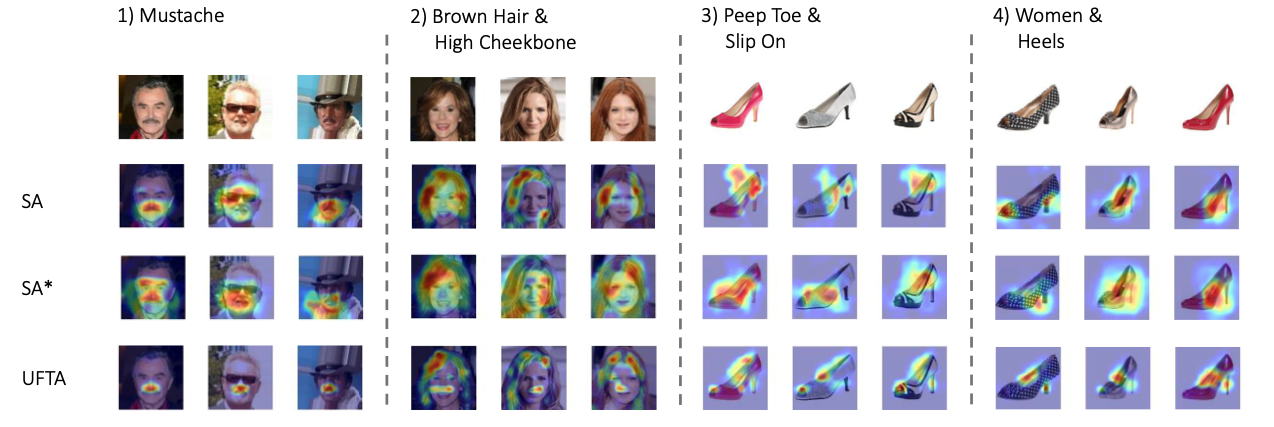
\includegraphics[width=6\textwidth]{figures/vis_cam_iccv.png}
\else
\ifarxiv
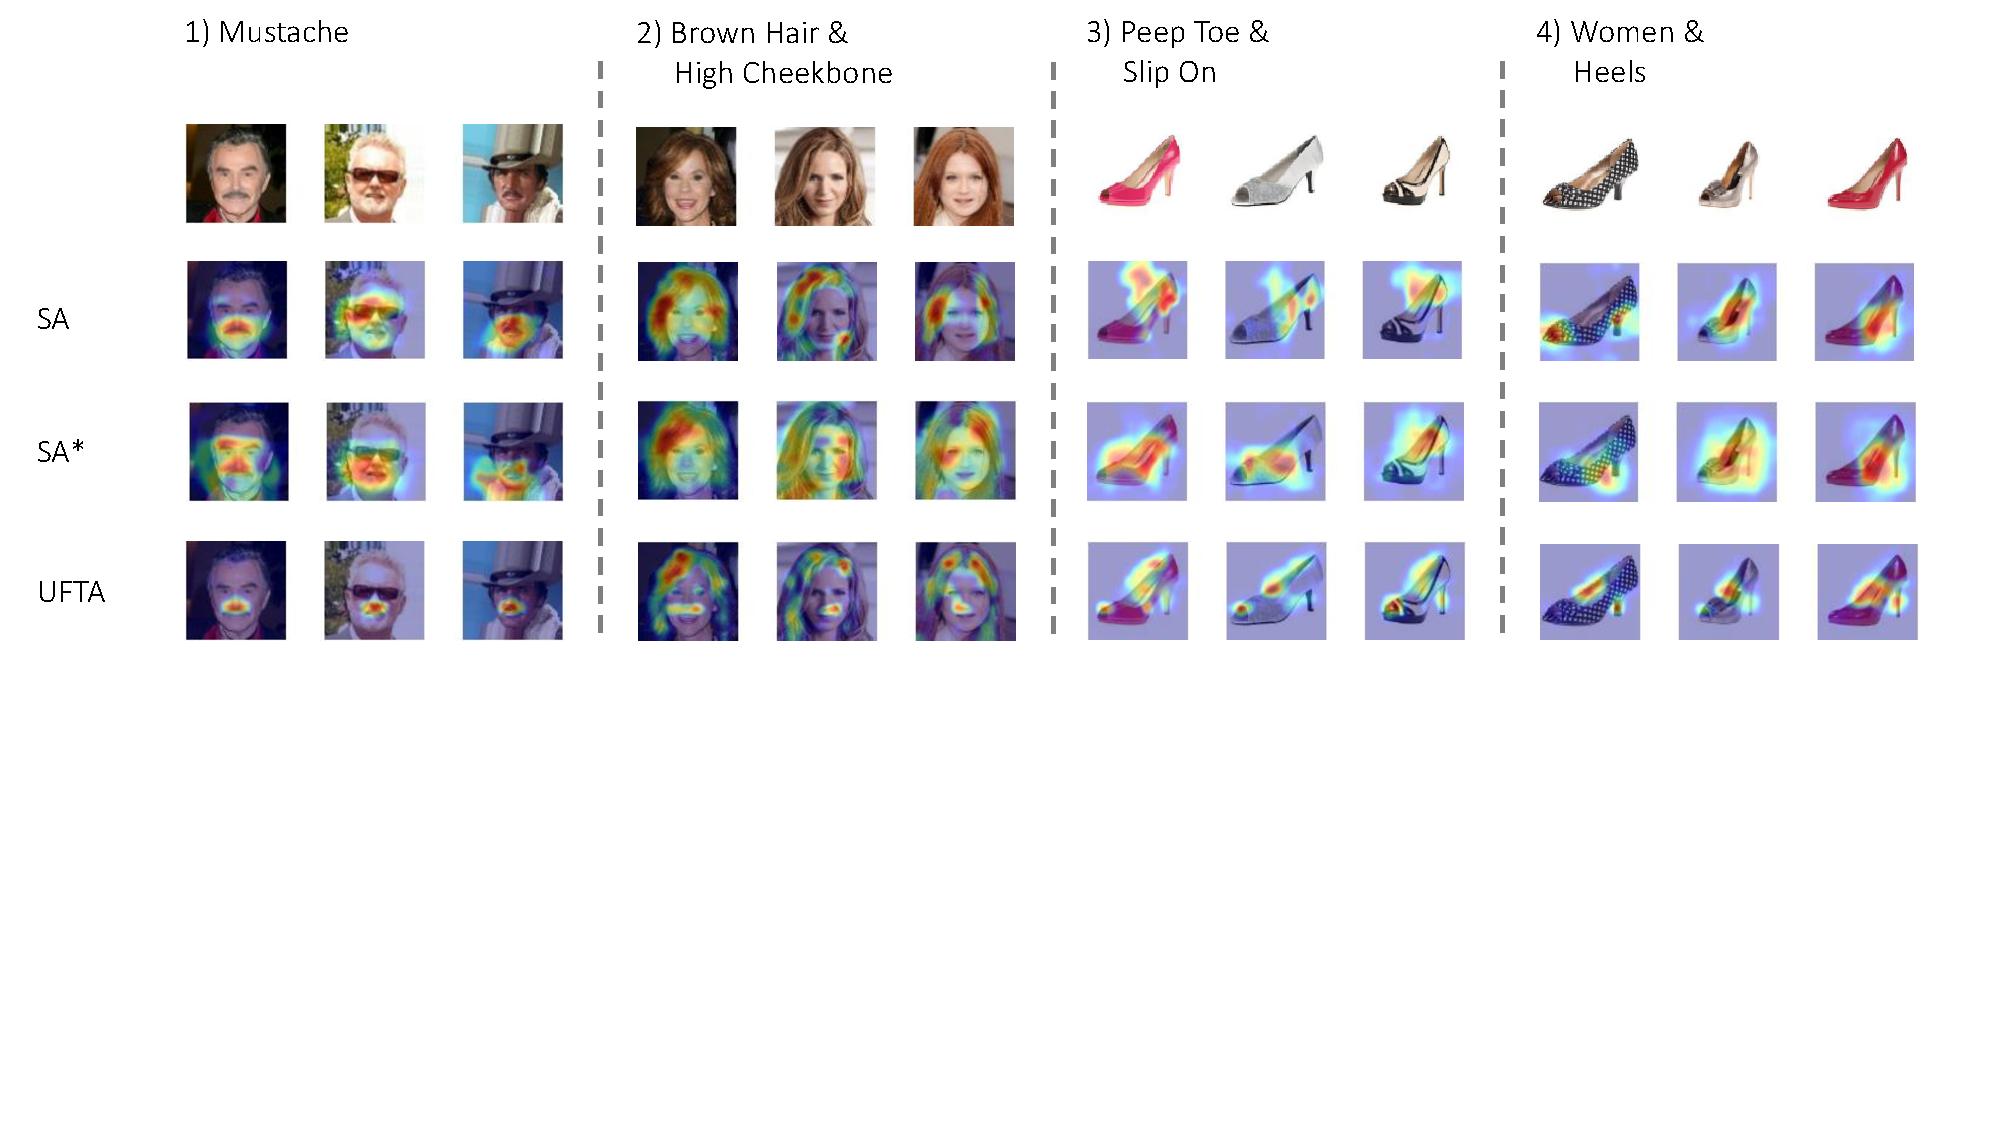
\includegraphics[width=\textwidth,trim={0 8cm 0
0.3cm},clip]{figures/vis_cam_iccv.pdf}
\else
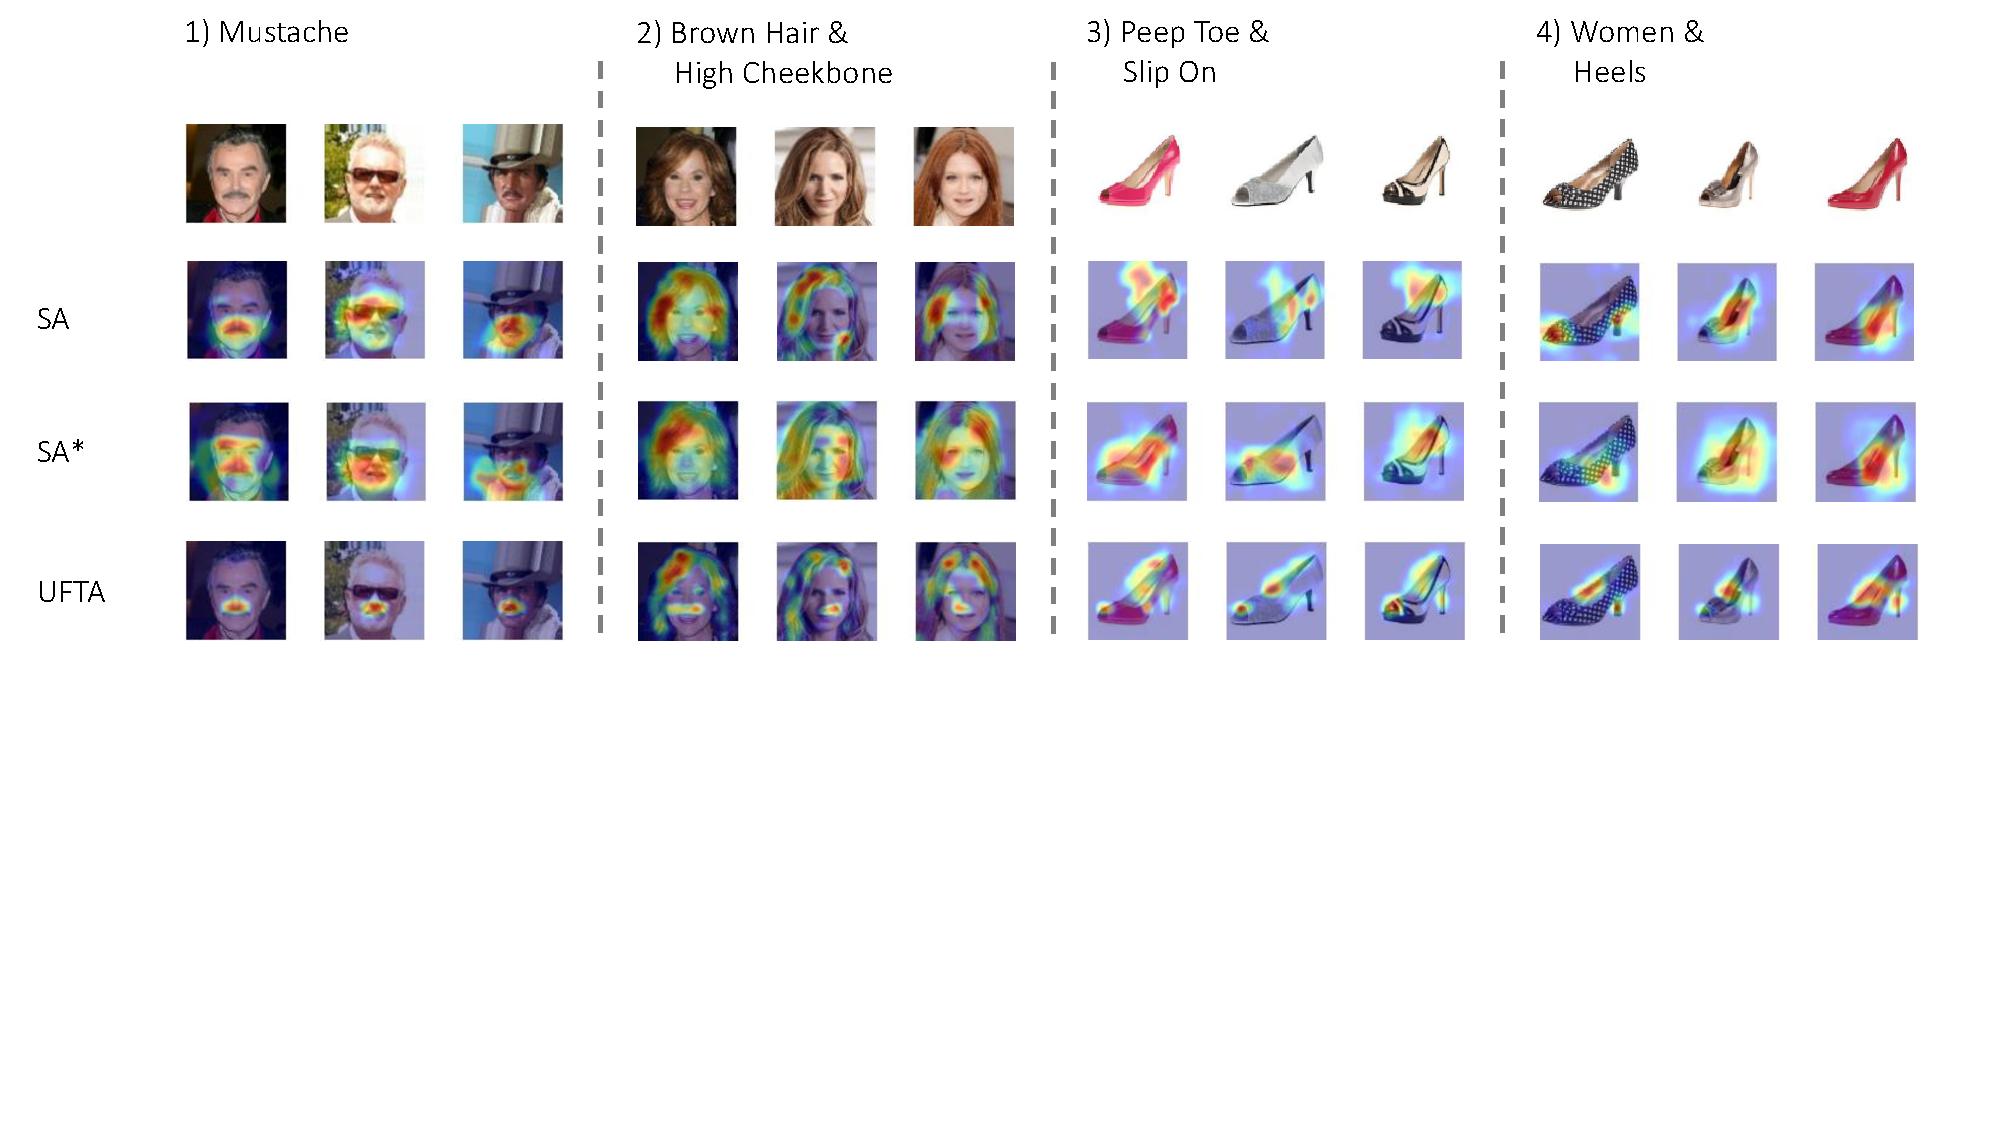
\includegraphics[width=\textwidth,trim={0 8cm 0
0.3cm},clip]{figures/vis_cam_iccv.pdf}
\fi
\fi
\savespacebeforesection
\savespacebeforesection
\caption{
\textbf{Visualization of few-shot classifiers using CAM~\citep{cam}, on top of
different representations.} Left: Celeb-A; Right: Zappos-50K. Target attributes
that define the episode are shown above and images are from the query set of
the positive class at test time.}
\label{fig:viz}
\savespacebeforesection
\savespacebeforesection
\end{figure*}

\iflatexml
\begin{figure}
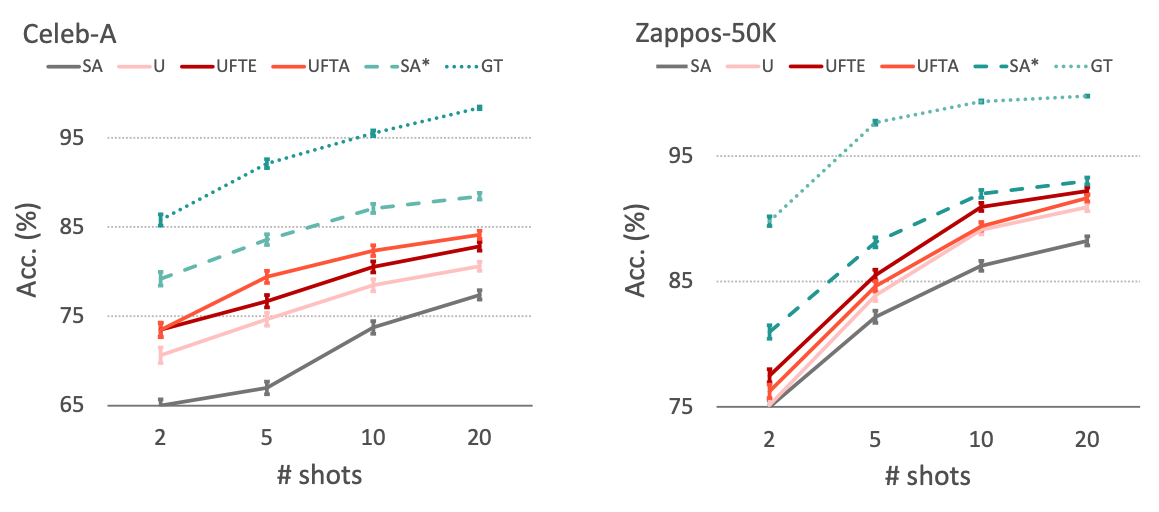
\includegraphics[width=6\textwidth]{figures/celeb-a-zappos-nshot.png}
\caption{\textbf{How many examples are needed for \taskname{}?} Performance
increases with number of shots, even when given the binary ground-truth
attribute vector (\textbf{GT}), suggesting that there is greater ambiguity in \taskname{} than in standard FSL.}
\label{fig:nshot}
\end{figure}

\begin{figure}
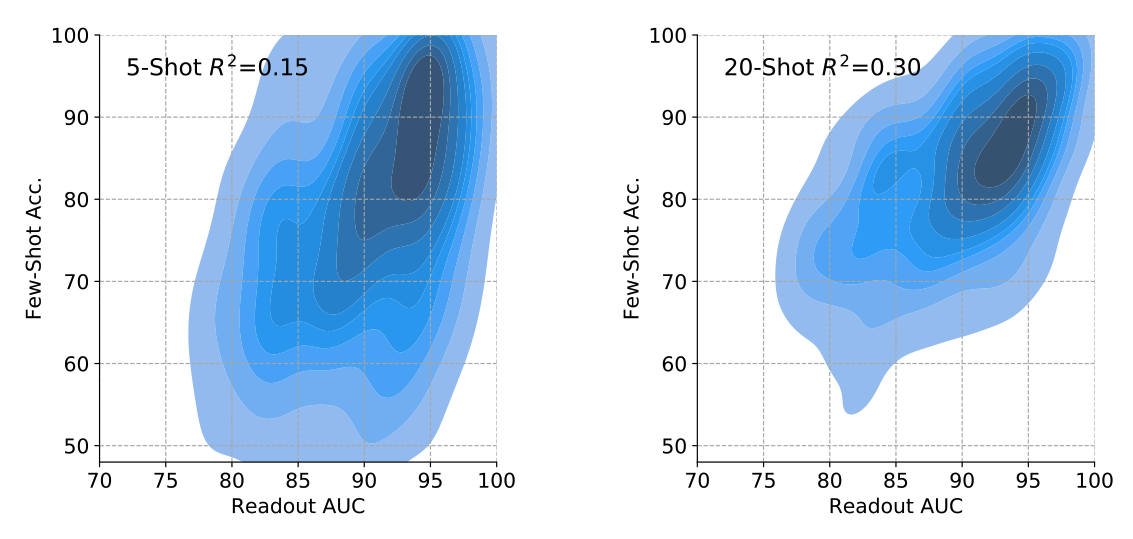
\includegraphics[width=6\textwidth]{figures/test-s5-s20.png}
\caption{\textbf{Correlation between readout AUC and few-shot acc. using
\uftsa}. Variance can be explained by the challenge of predicting attributes
and the ambiguity of \taskname{}. More shots reduce variance and improve
correlation.}
\label{fig:corr}
\end{figure}

\else

\begin{figure*}[t]
\savespacefigtop{-0.5in}
\centering
\begin{minipage}[b]{0.49\textwidth}
\centering
\ifarxiv
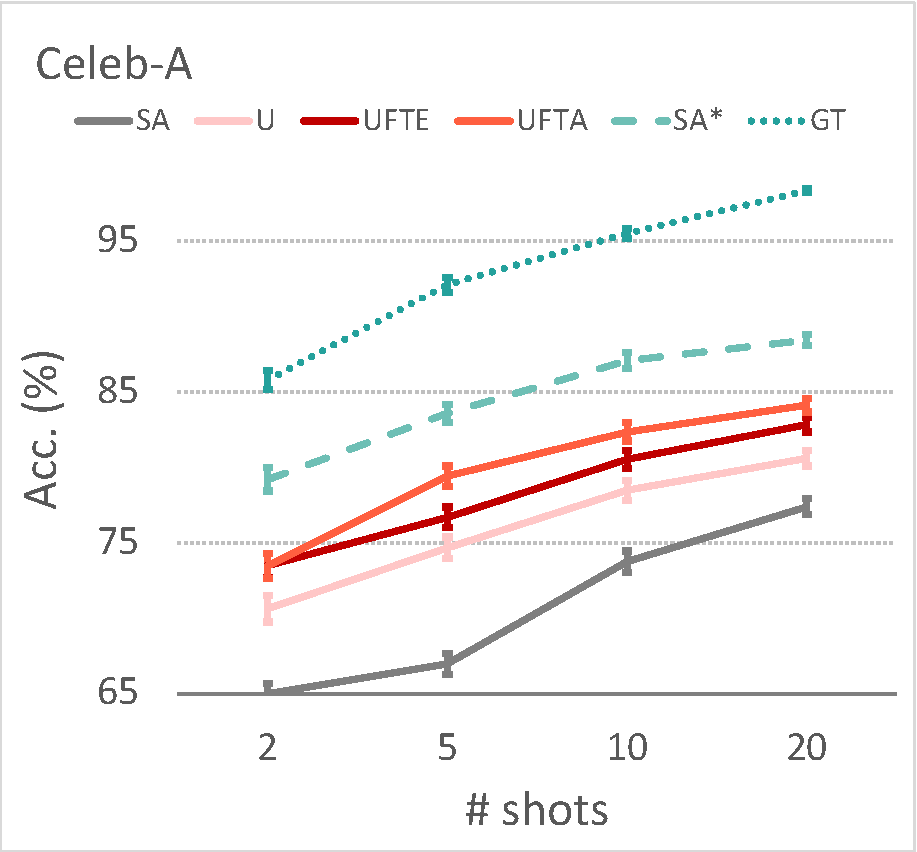
\includegraphics[height=3.1cm,trim={0.2cm 0.2cm 0.2cm 0.2cm},clip]{figures/celeb-a-nshot-v3.pdf}
\quad
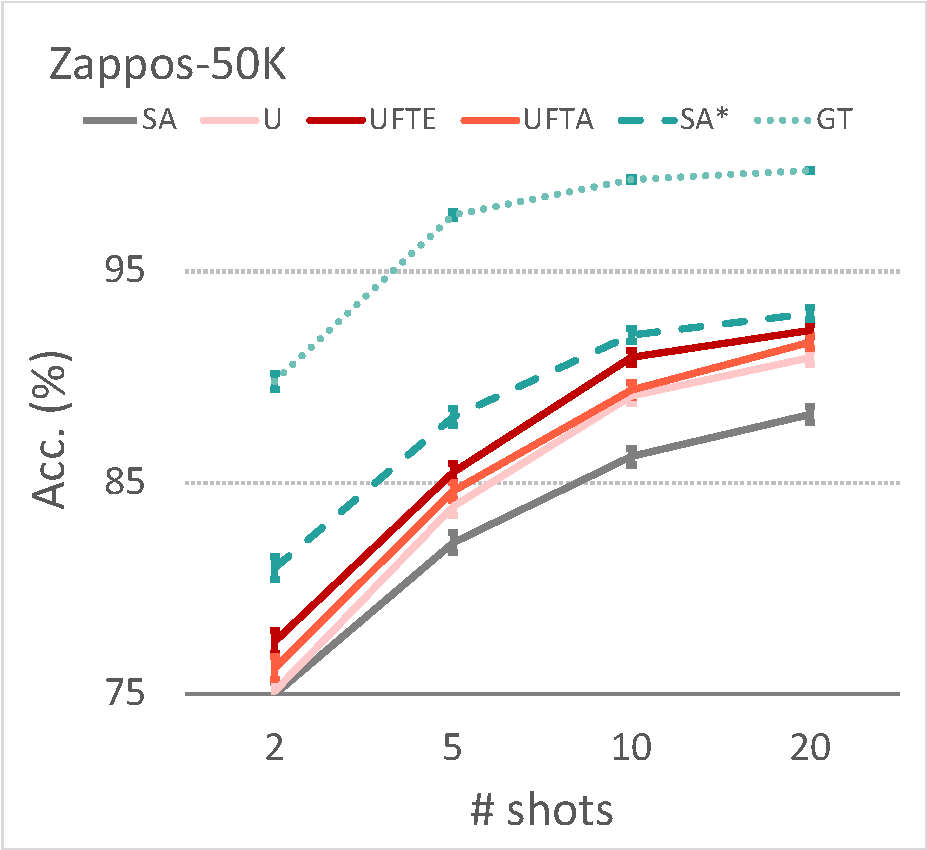
\includegraphics[height=3.1cm,trim={0.2cm 0.2cm 0.2cm 0.2cm},clip]{figures/zappos-nshot-v4.pdf}
\else
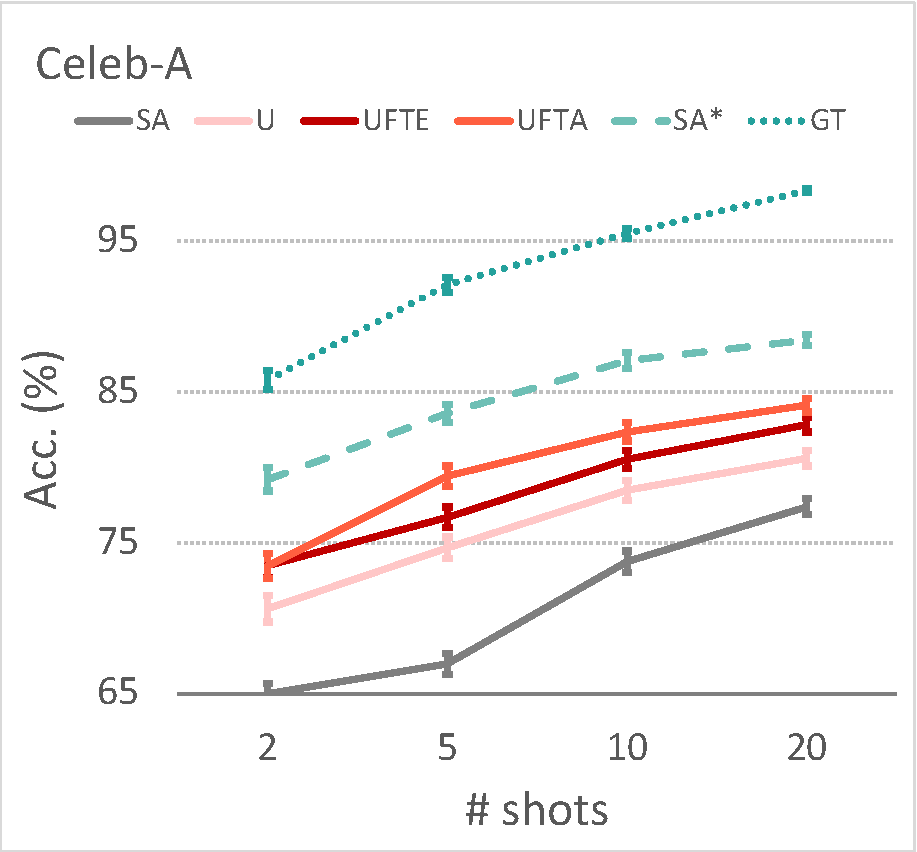
\includegraphics[height=2.8cm,trim={0.2cm 0.2cm 0.2cm 0.2cm},clip]{figures/celeb-a-nshot-v3.pdf}
\quad
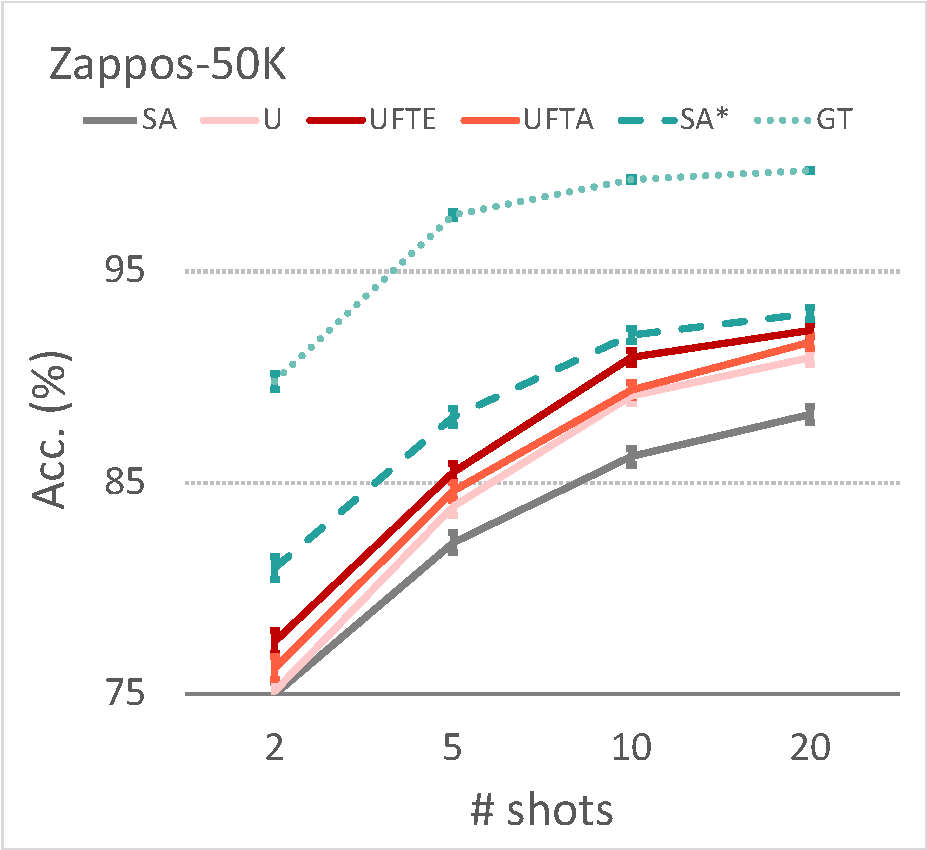
\includegraphics[height=2.8cm,trim={0.2cm 0.2cm 0.2cm 0.2cm},clip]{figures/zappos-nshot-v4.pdf}
\fi
\savespacebeforesection
\caption{\textbf{How many examples are needed for \taskname{}?} Performance
increases with number of shots, even when given the binary ground-truth
attribute vector (\textbf{GT}), suggesting that there is greater ambiguity in \taskname{} than in standard FSL.}
\label{fig:nshot}
\end{minipage}
\hfill
\begin{minipage}[b]{0.49\textwidth}
\centering
\ifarxiv
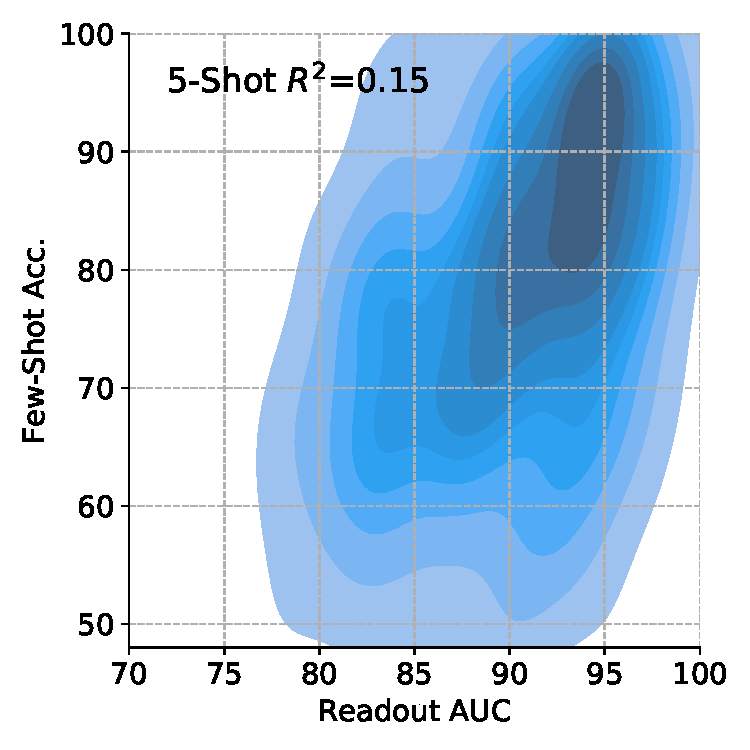
\includegraphics[height=3.3cm]{figures/test-s5.pdf}
\quad
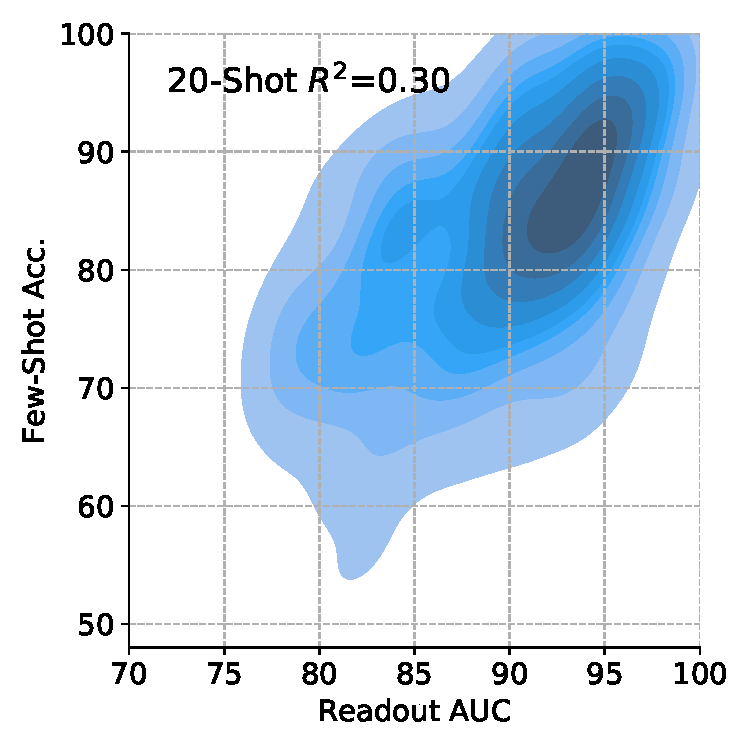
\includegraphics[height=3.3cm]{figures/test-s20.pdf}
\else
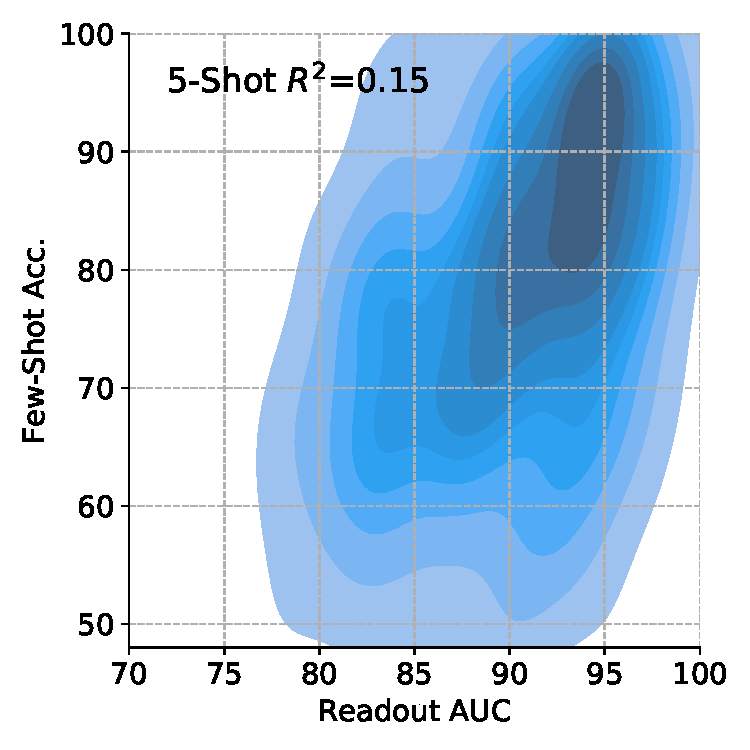
\includegraphics[height=3.0cm]{figures/test-s5.pdf}
\quad
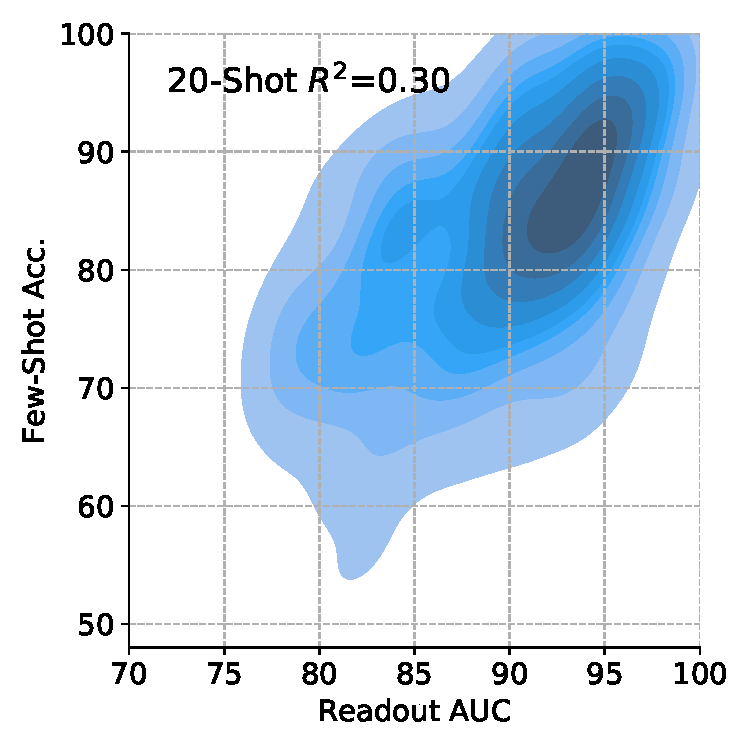
\includegraphics[height=3.0cm]{figures/test-s20.pdf}
\fi
\vspace{-0.08in}\savespacebeforesection
\caption{\textbf{Correlation between readout AUC and few-shot acc. using \uftsa}. Variance can be explained by the challenge of predicting attributes
and the ambiguity of \taskname{}. More shots reduce variance and improve correlation.}
\label{fig:corr}
\end{minipage}
\vspace{-0.15in}
\end{figure*}

\fi



\savespacebeforesection
\subsection{Comparing Various Methods for \taskname{}}
\savespacebeforesection
\label{sec:experiments:results}

Table~\ref{tab:main} shows our main results on Celeb-A and Zappos-50K with 5-
and 20-shot episodes. Table~\ref{tab:combo} explores different combinations of
representations and few-shot learners. Overall, the standard episodic
meta-learners performed relatively poorly. Also, supervised attribute (SA)
learning and learning via the auxiliary task of class facial identification
(ID) were not helpful for representation learning either. Interestingly, U
attained relatively better test performance, suggesting that the training
objective in contrastive learning indeed preserves more general features---not
just for semantic classification tasks as shown in prior work, but also for the
flexibly-defined attribute classes in our FSAL paradigm. All these evidences suggest that unsupervised representation learning is better than supervised methods for FSAL. 

Moreover, \uftsa{} and \uftpn{} approaches obtained significant gains in
performance, suggesting that a combination of unsupervised features with some
supervised information is indeed beneficial for this task. Lastly, they
are able to reduce the generalization gap between SA and the oracle SA*, in
fact almost closing it entirely on Zappos-50K. We investigate and analyze the benefit of unsupervised pretraining and supervised finetuning further in Section~\ref{sec:analysis}.

Results on ImageNet-with-Attributes are reported separately for clarity,
because U, \uftpn{}, and \uftsa{} had access to additional unlabeled examples.
As shown in Table~\ref{tab:imagenet-main}, both \uftpn{} and \uftsa{}
outperformed other methods substantially. Because of the additional unlabeled
data available in this setting, even U achieved a substantially better accuracy
than SA and MAML. Results in Table~\ref{subtab:imagenet-fsl} show that \uftpn{}
and \uftsa{} work well when combined with different few-shot learners.

\savespacebeforesection
\looseness=-10000
\paragraph{Visualizing few-shot classifiers:} To understand and interpret the
decision made by few-shot linear classifiers, we visualize the classifier
weights by using CAM~\citep{cam}, and plot the heatmap over the 11$\times$11
spatial feature map in Figure~\ref{fig:viz}. SA sometimes shows incorrect
localization as it is not trained to classify those novel test attributes. SA*
shows bigger but less precise heatmaps since the training objective encourages
the propagation of attribute information spatially. In contrast, UFTA produces
accurate and localized heatmaps that pinpoint the location of the attributes
(e.g. mustache or cheekbone); this is impressive since no labeled information
concerning these attributes was available during representation pre-training
and finetuning. This result supports the hypothesis that local features can be
good descriptors that match different views of the same instance during
contrastive learning, and finetuning further establishes a positive transfer
between training and test attributes.

\savespacebeforesection
\paragraph{Number of shots and task ambiguity:} 
Our few-shot attribute learning episodes can be ambiguous. For example, by
presenting only a smiling face with eyeglasses in the support set, it is
unclear whether the positive set is determined by ``smiling'' or ``wearing
eyeglasses''. Figure~\ref{fig:nshot} show several approaches evaluated using LR
with varying numbers of support examples per class in Celeb-A and Zappos-50K
episodes, respectively. The oracle GT gradually approached 100\% accuracy as
the number of shots approached 20. This demonstrates that \taskname{} tasks
potentially require more support examples than standard FSL to resolve
ambiguity. Again here, \uftsa{} and \uftpn{} consistently outperformed U, SA,
and ID across different number of shots. Figure~\ref{fig:corr} shows the
correlation between readout performance of attributes and few-shot learning
accuracy, using \uftsa{}. With a larger number of shots, there is a higher
correlation between the two, but there is still a large amount of variance that
is due to the ambiguity of the task itself. More details are included in the
Appendix.

\savespacebeforesection
\paragraph{Ablation studies:} Table~\ref{tab:projection} studies the effect of
the projection MLP for attribute classification finetuning. Adding MLP
projection layers was found to be beneficial for unsupervised learning in prior
work~\citep{simclr}. Here we found that adding MLP layers is also critical in
supervised finetuning. Finetuning directly on the
backbone (depth=0), and keeping the MLP during test (Discard=no) both led to
significant drop in performance. In the Appendix, we also report on studies of
the effect of adding the L1 regularizer on LR.

\savespacebeforesection
\subsection{Analysis of Few-Shot Generalization}
\label{sec:analysis}
\savespacebeforesection
In Tables~\ref{tab:gap} and \ref{subtab:imagenet-traintest-gap}, we study the
performance gap between training attributes and test attributes. Notably, SA
performs very well on test episodes defined using training attributes, but
there is a large generalization gap between training and test attributes.
\uftpn{} and \uftsa{} show significant improvements in terms of reducing the
generalization gap between training and test attributes. Moreover, we find that
self-supervised pre-training generally preserves informative features and is
more general than supervised pre-training.

\savespacebeforesection
\paragraph{Investigating the cause of generalization issues:} 
\looseness=-1
We hypothesize that the weak performance of episodic learners and SA on our
benchmarks is because their training objectives essentially encourage ignoring
attributes that are not useful at training time, but may still be useful at
test time. In Appendix~\ref{app:toy_problem}, we study a synthetic problem to
further analyze these generalization issues. We explore training a ProtoNet
model on data from a linear generative model, where each FSAL episode presents
ambiguity in identifying the relevant attributes. In this setting, the network
is forced to discard information that is useful for test tasks to solve the
training tasks effectively, and thus fails to generalize.

\begin{figure*}[t]
\savespacefigtop{-0.5in}
\centering
% \ifarxiv
\iflatexml
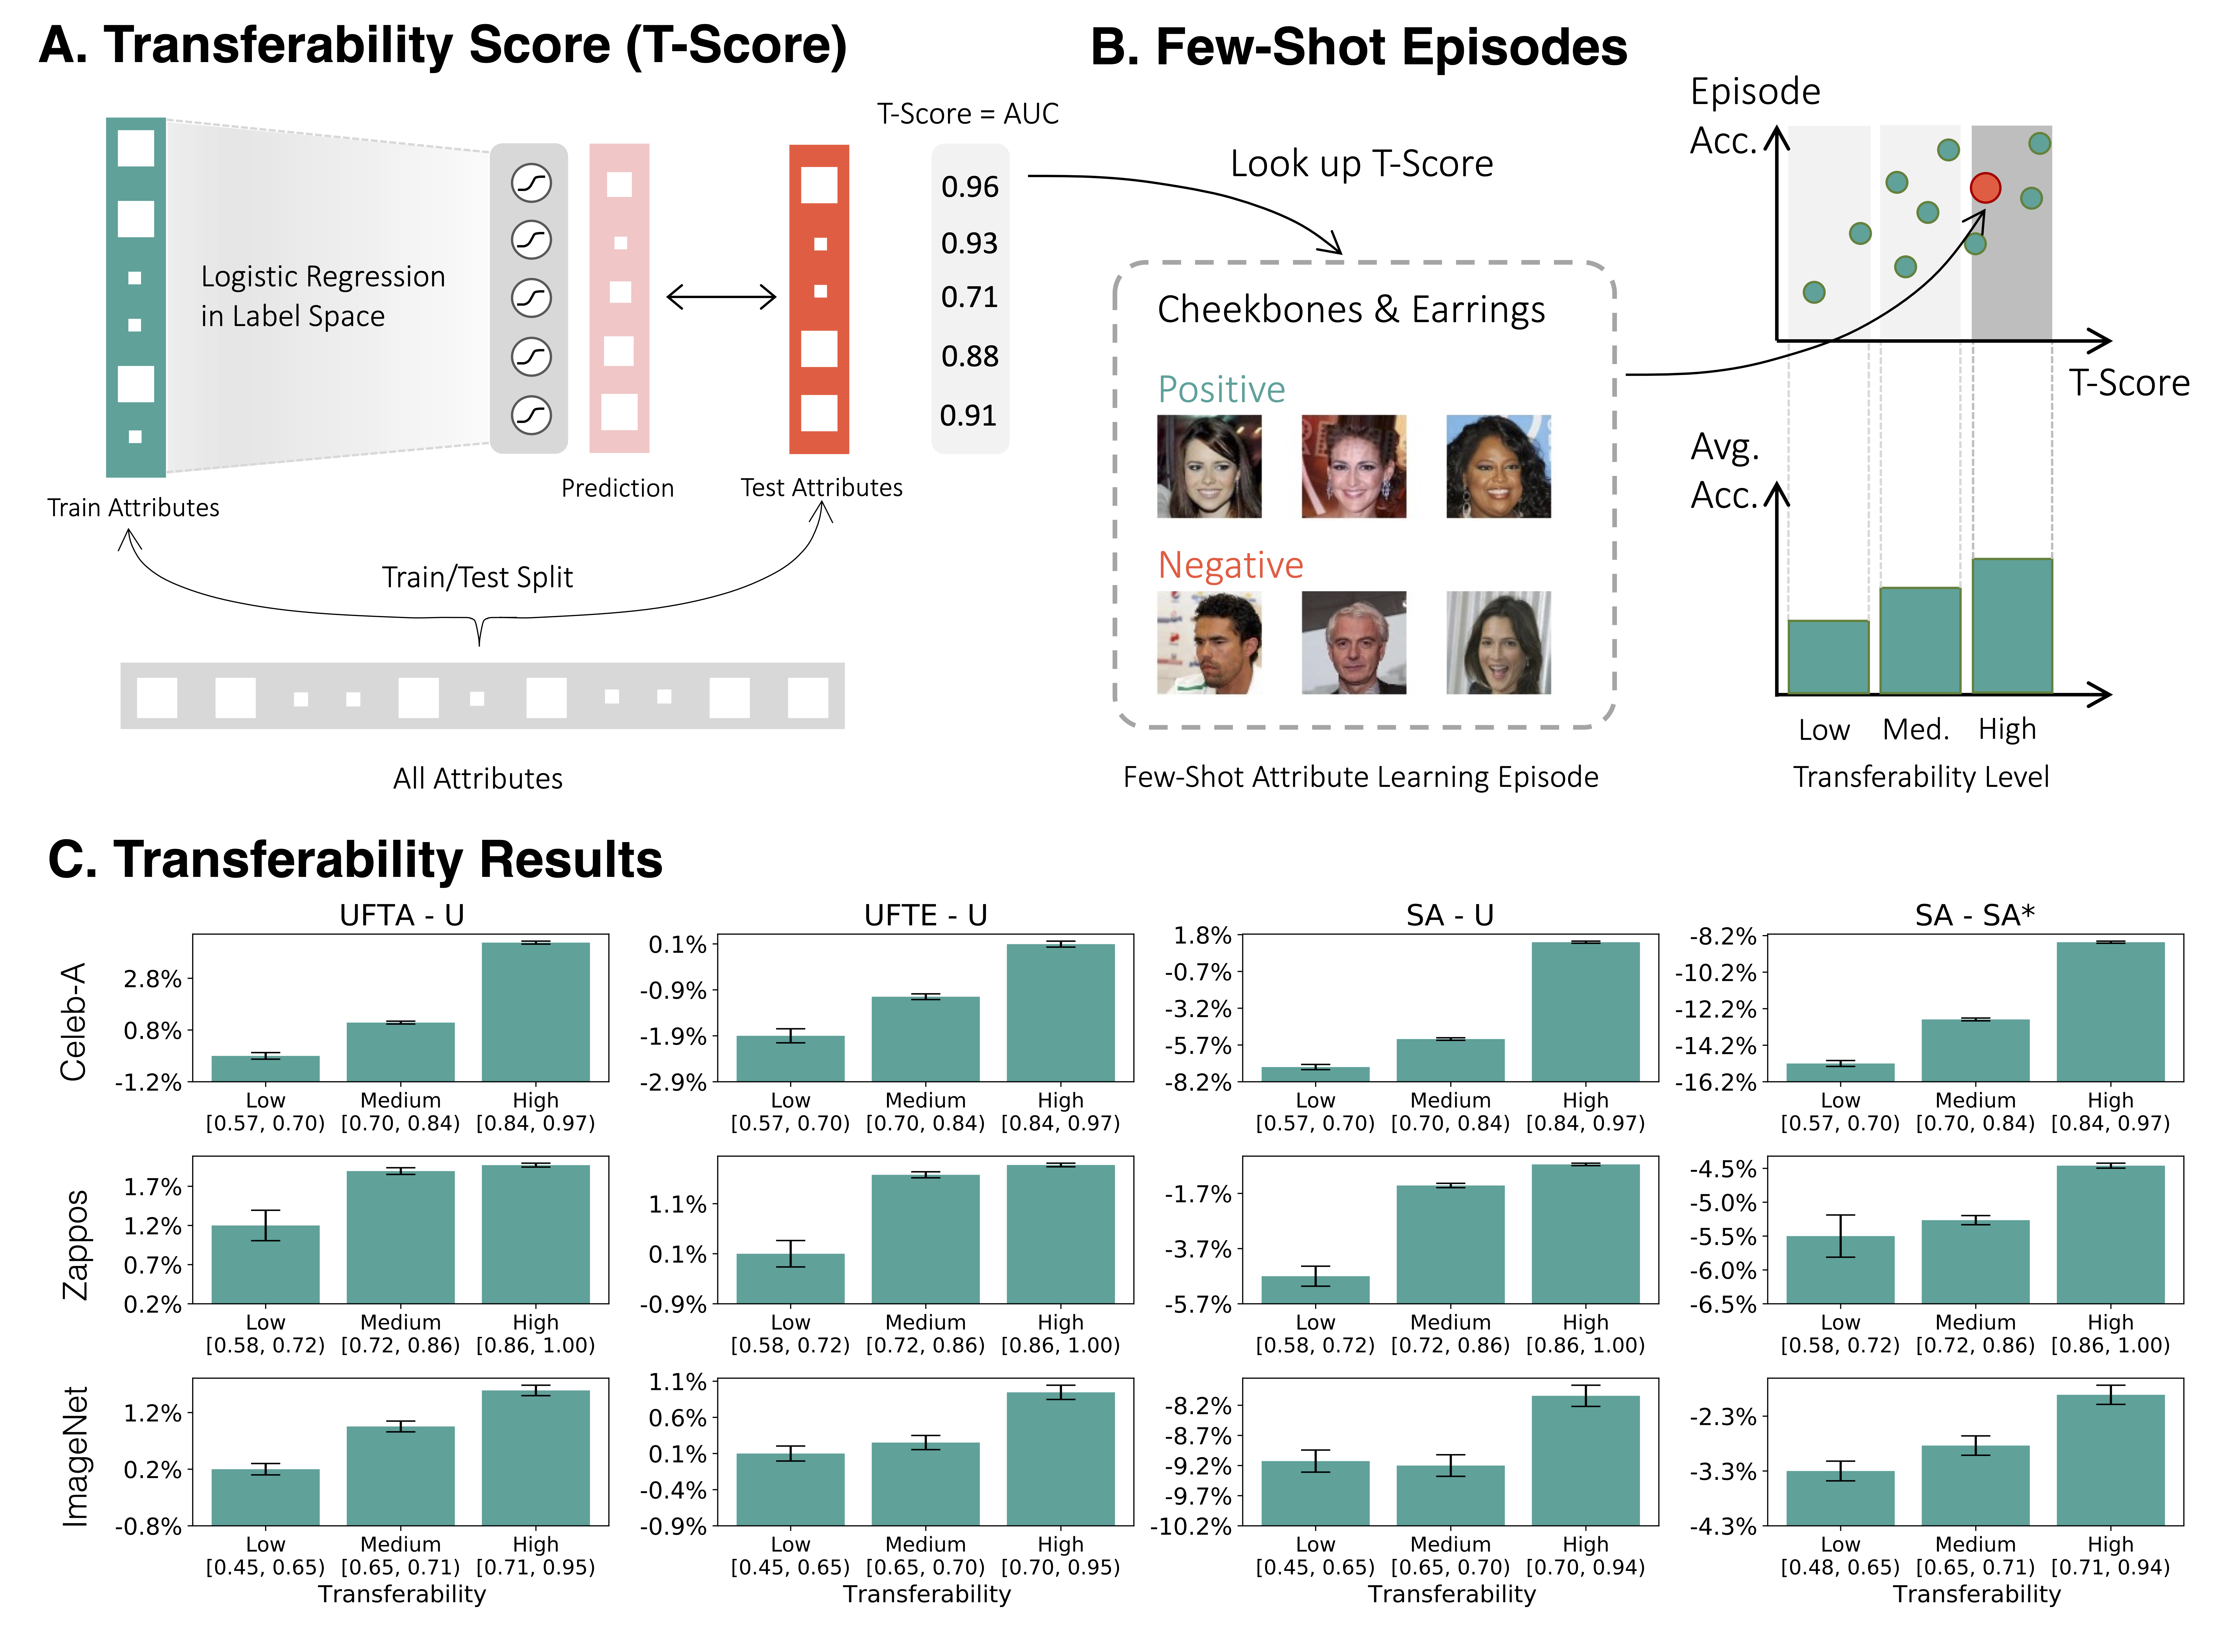
\includegraphics[width=6\textwidth]{./figures/transferability_combo.png}
\else
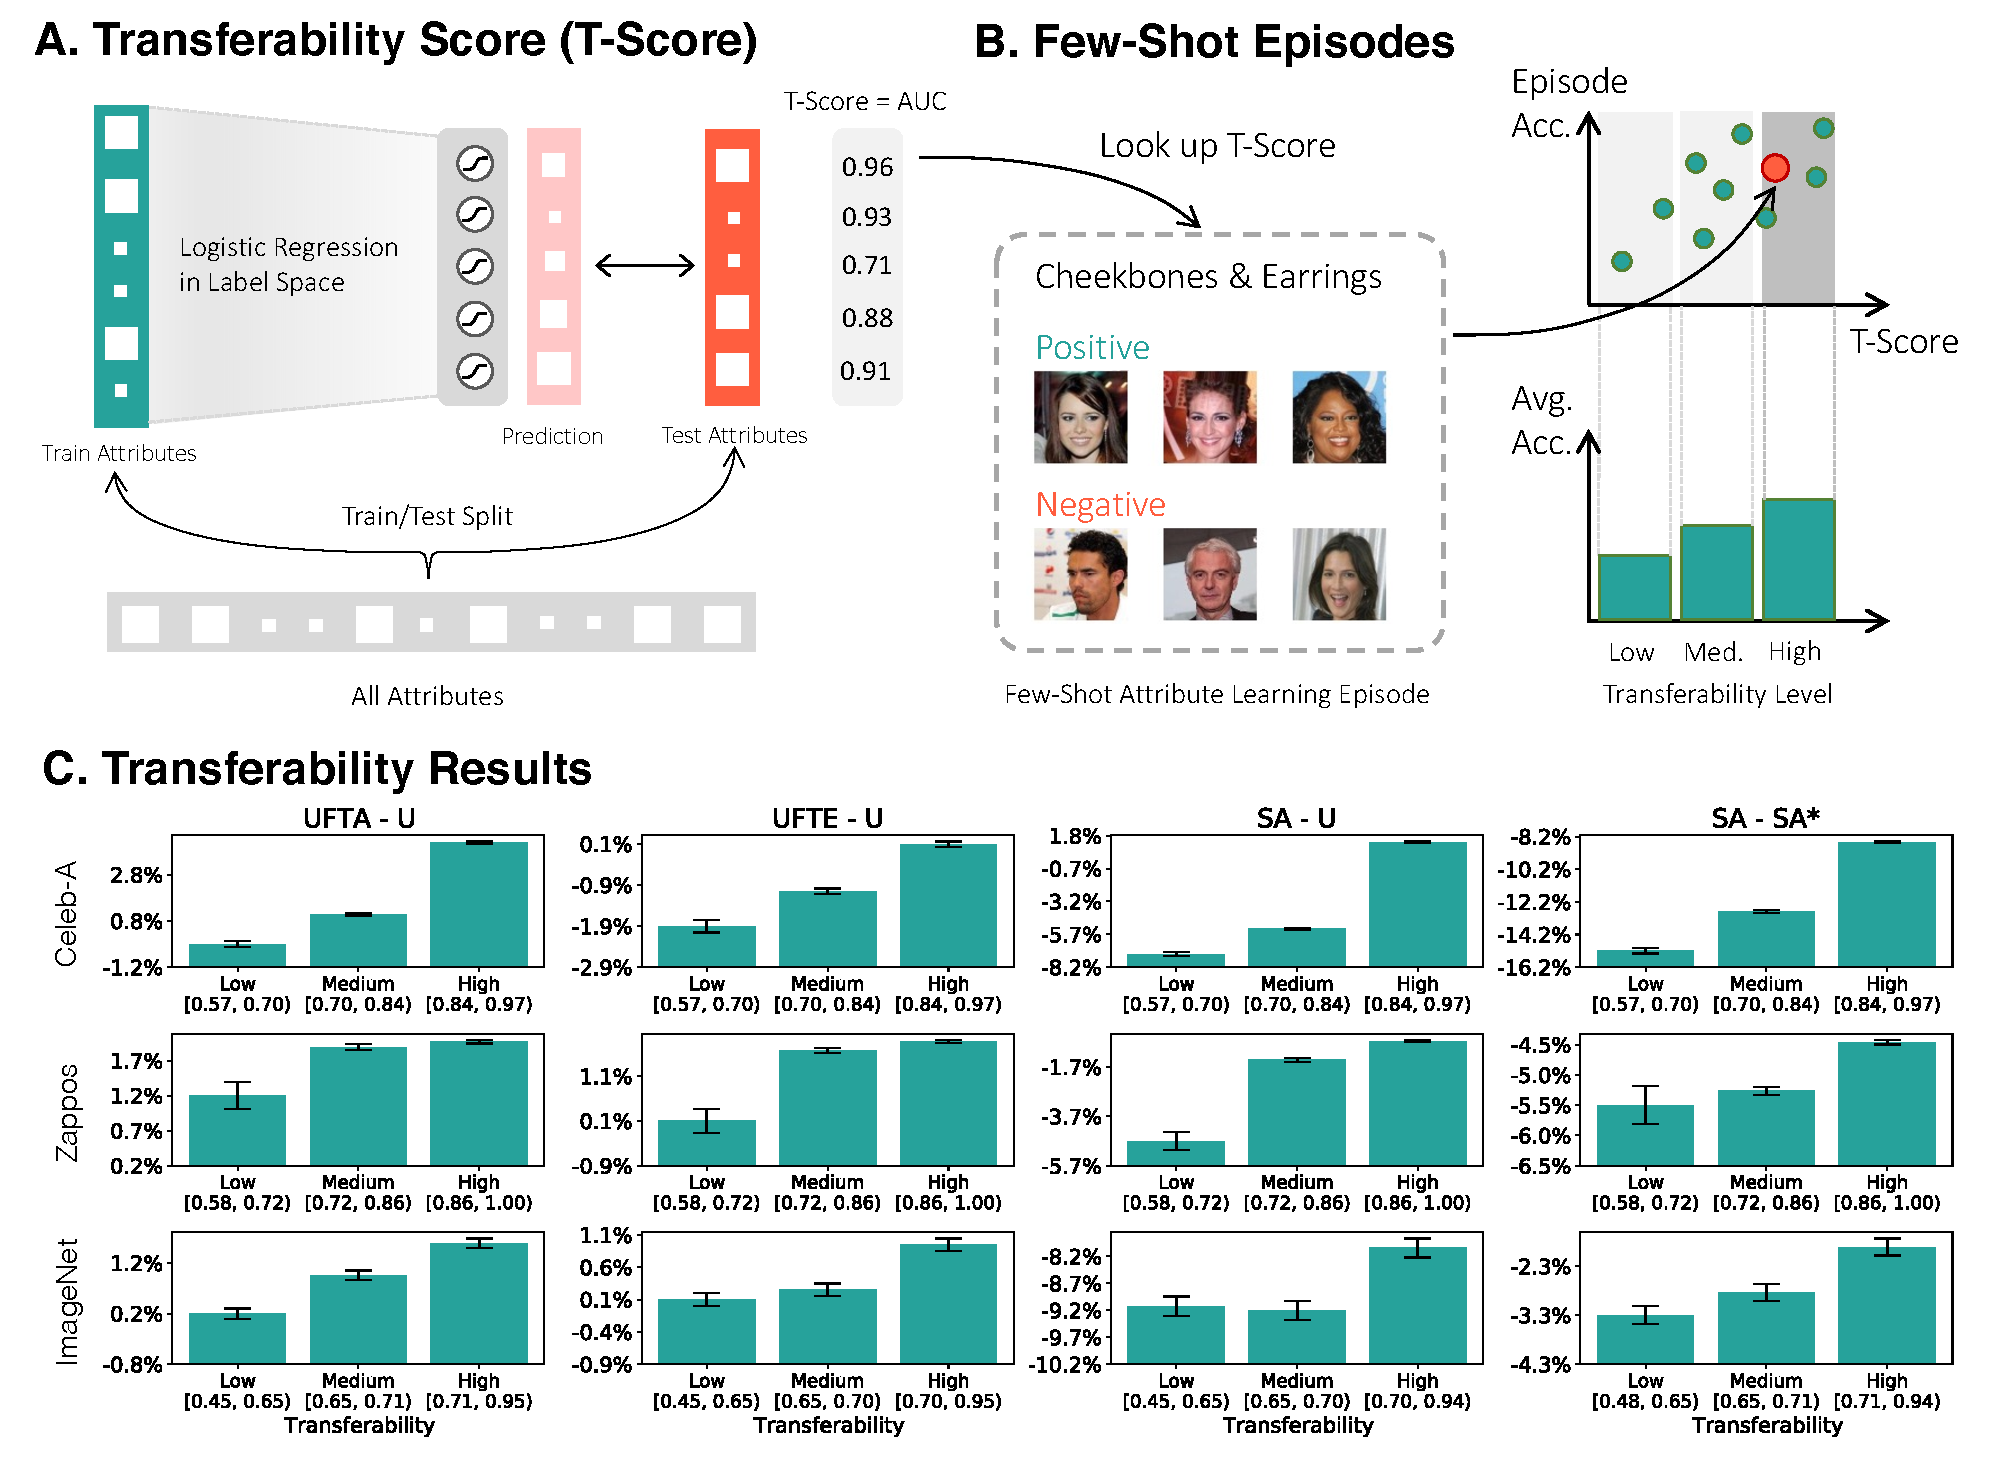
\includegraphics[width=\textwidth]{./figures/transferability_combo.pdf}
\fi
% \else
% 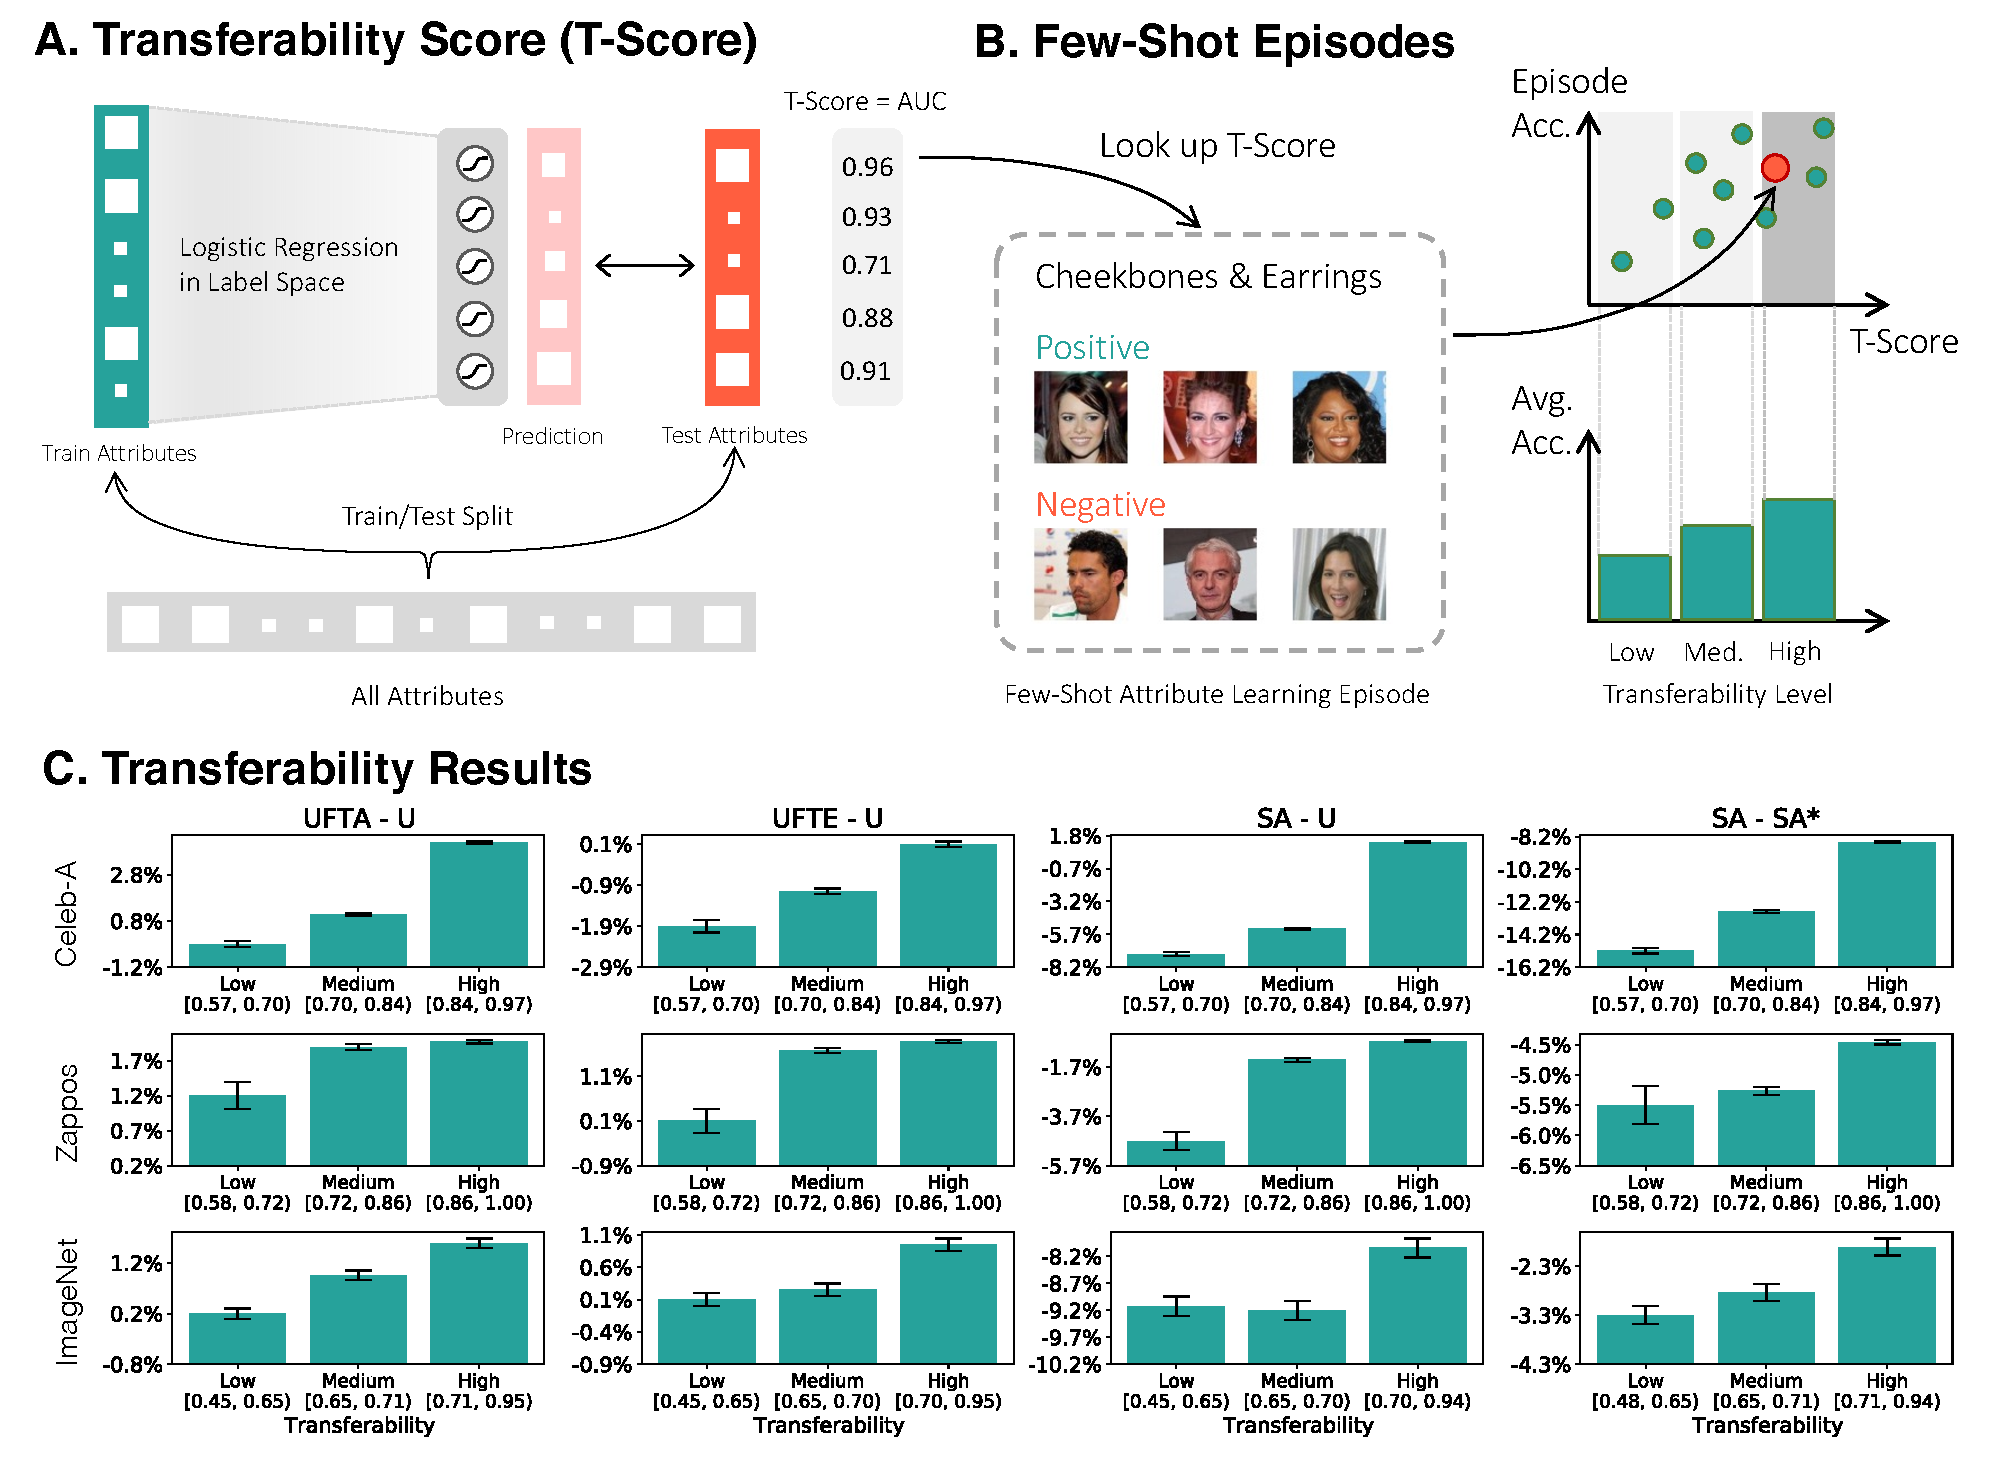
\includegraphics[width=0.9\textwidth]{./figures/transferability_combo.pdf}
% \fi
\savespacebeforesection
\savespacebeforesection
\savespacebeforesection
\caption{
\looseness=-10000
\textbf{Few-shot performance vs. transferability across training and test
attributes.} \textbf{A:} Transferability score (T-score) is computed based on
the AUC of a test attribute predicted by a logistic regression model on a set
of training attributes. 100 different random splits across train/test
attributes per split are used. \textbf{B:} Both episodic accuracy and T-scores
are recorded on 60,000 episodes (600 episodes per split). Episodes are grouped
into three bins by their T-scores. \textbf{C:} Performance of training or
finetuning on training attributes correlates with T-score. Error bars are
standard errors in each bin.}
\label{fig:transfer}
\savespacebeforesection
% \savespacebeforesection
% \vspace{-0.15in}
\savespacebeforesection
\end{figure*}

\savespacebeforesection
\paragraph{Transferability score:}
\looseness=-1000
We aim to investigate the question of why unsupervised pretraining and
supervised finetuning produce better performance, and whether the performance
difference is caused by the closeness between training and test attributes.
More concretely, we aim to predict the transferability between training and
test splits by analyzing the training vs. test attributes. Each image has a
complete attribute vector, describing the values of each attribute in the
image. Some of these attributes are in the training set, and others in the test
set. To quantify the transferability, we leverage the idea of mutual
information. In particular, we learn a logistic regression model that takes the
training attribute vector in a particular image as input and predicts the value
of one of the test attributes in that image. Each logistic regression model
will generate an AUC score on held-out images, and we average them across the
relevant test attributes in each episode, and we define this AUC score as the
``transferability score.'' Our hypothesis is that more mutual information
between the attribute label distributions will translate to higher transfer
performance.

In Figure~\ref{fig:transfer}, we ran experiments using 100 random splits of
training and test attributes. The results verify our hypothesis. We see
positive correlation between the transfer performance and our transferability
score: When subtracting U as a baseline, both UFTA and UFTE models get better
when there is higher transferability (subtraction reduces the effect of
per-episode variability). The same conclusion can be drawn when we subtract SA*
from SA. By plotting the relation between U and SA, we show that supervised
learning is more helpful when there is higher transferability in the label
space whereas self-supervised learning is more flexible at adapting to novel
target tasks.

\looseness=-10000
To summarize, our empirical evidence suggests that unsupervised representation
learning is superior to supervised methods in terms of retaining information
relevant to the test attributes. Other methods, such as supervised
representation learning or episodic training, tend to effectively ignore
attributes that were not used for labelling during training. Moreover,
supervised finetuning of the representations is helpful when the
transferability between test and train attributes is high, but less so
otherwise, and supervised pretraining alone is harmful to novel attribute
generalization for most train vs. test attribute pairs.
